\chapter{Design}
\section{Main Screens}
This chapter will describe the design decision for each of the screens that can be reached within the app. Each subsection will address how the design progressed over time and any alternative designs considered. Each screen's final design is justified through also analysing its benefits and limitations. In order, the main screens analysed below are:
\begin{enumerate}
    \item \textbf{Body Screen} - App home screen for body part selection 
    \item \textbf{Information Screens} - Tutorial screen for first time users
    \item \textbf{Old Spot Screen} - List of spots added to a chosen body part
    \item \textbf{Camera and Cropping Screen} - Screens used to add new spot photos
    \item \textbf{Spot Naming Screen} - Screen to name a new spot to be saved
    \item \textbf{Spot Image List Screen} - List of all photos taken of a spot
    \item \textbf{Comparing Spots Screen} - Comparison screen for two side by side spot images
    \item \textbf{Email Screen} - Screen for emailing selected images to a doctor
    
\end{enumerate}

\subsection{Body Screen}
This screen acts as the app homepage, it is the first screen displayed to the user (excluding the first time use tutorial). This screen is the result of a series of design refactors that occured within the first few weeks of development. These are explained in depth in section \ref{nav_refactor}. 

The final design for the body screen is displayed in figure \ref{fig:bodyfinalscreen}. The toolbar includes an "i" button, which refers the user to the information screens (Section \ref{sec:infoscreens}). Pressing a body part button such as "Right Arm" would take the user to the O
old spot list screen (Section \ref{sec:oldspotscreen}). To switch between the front and back body perspectives, the user can simply swipe the screen or tap the "front" and "back" body tabs.

Designs for the actual body image changed throughout the whole duration of the project. This came as a result of beta testing, usability tests and preference tests. The evolution of the screen is displayed in figures \ref{fig:it1design}-\ref{fig:it15design}. Designs are numbered 1-5 and a short justification for each approach is included below.
\begin{enumerate}
    \item Design Iteration 1 - Used as a placeholder for the eventual official screen, this image was simply used as a background to make the app more graphical during early stages of development. The same image was used for front and back.
    \item Design Iteration 2 - Due to limited artistic skills, a decision was made to find an external source for the body images. After browsing through the iStock photo library (Service offering copyright free images), this body outline was chosen. It provided a back and front side perspective with a simple, clean look. Consent was requested through the university's image graphic design department.
    \item Design Iteration 3 - Getting closer to the final design, the changes to this design had the goal of making the image and app more gender neutral, this was done by widening the hips and removing the pectoral marks. This process required learning and using \emph{Inkscape} (Vector graphics editor).
    \item Design Iteration 4 - It was decided to add some indication of where the app separates body parts, this would become important if the buttons were hidden, and it would make it even more clear that spots are saved under different body parts.
    \item Design Iteration 5 - At this stage, there was the idea of adding color to the different body parts, indicating the separations even more, and replicating the design of an unfinished prototype app by Maunik Desai. The choice of which final design to use would be left in the hands of end-users, this would be done via usability evaluations and preference testing.
\end{enumerate}

\begin{figure*}[t!]
    \centering
    \begin{subfigure}[t]{0.5\textwidth}
        \centering
        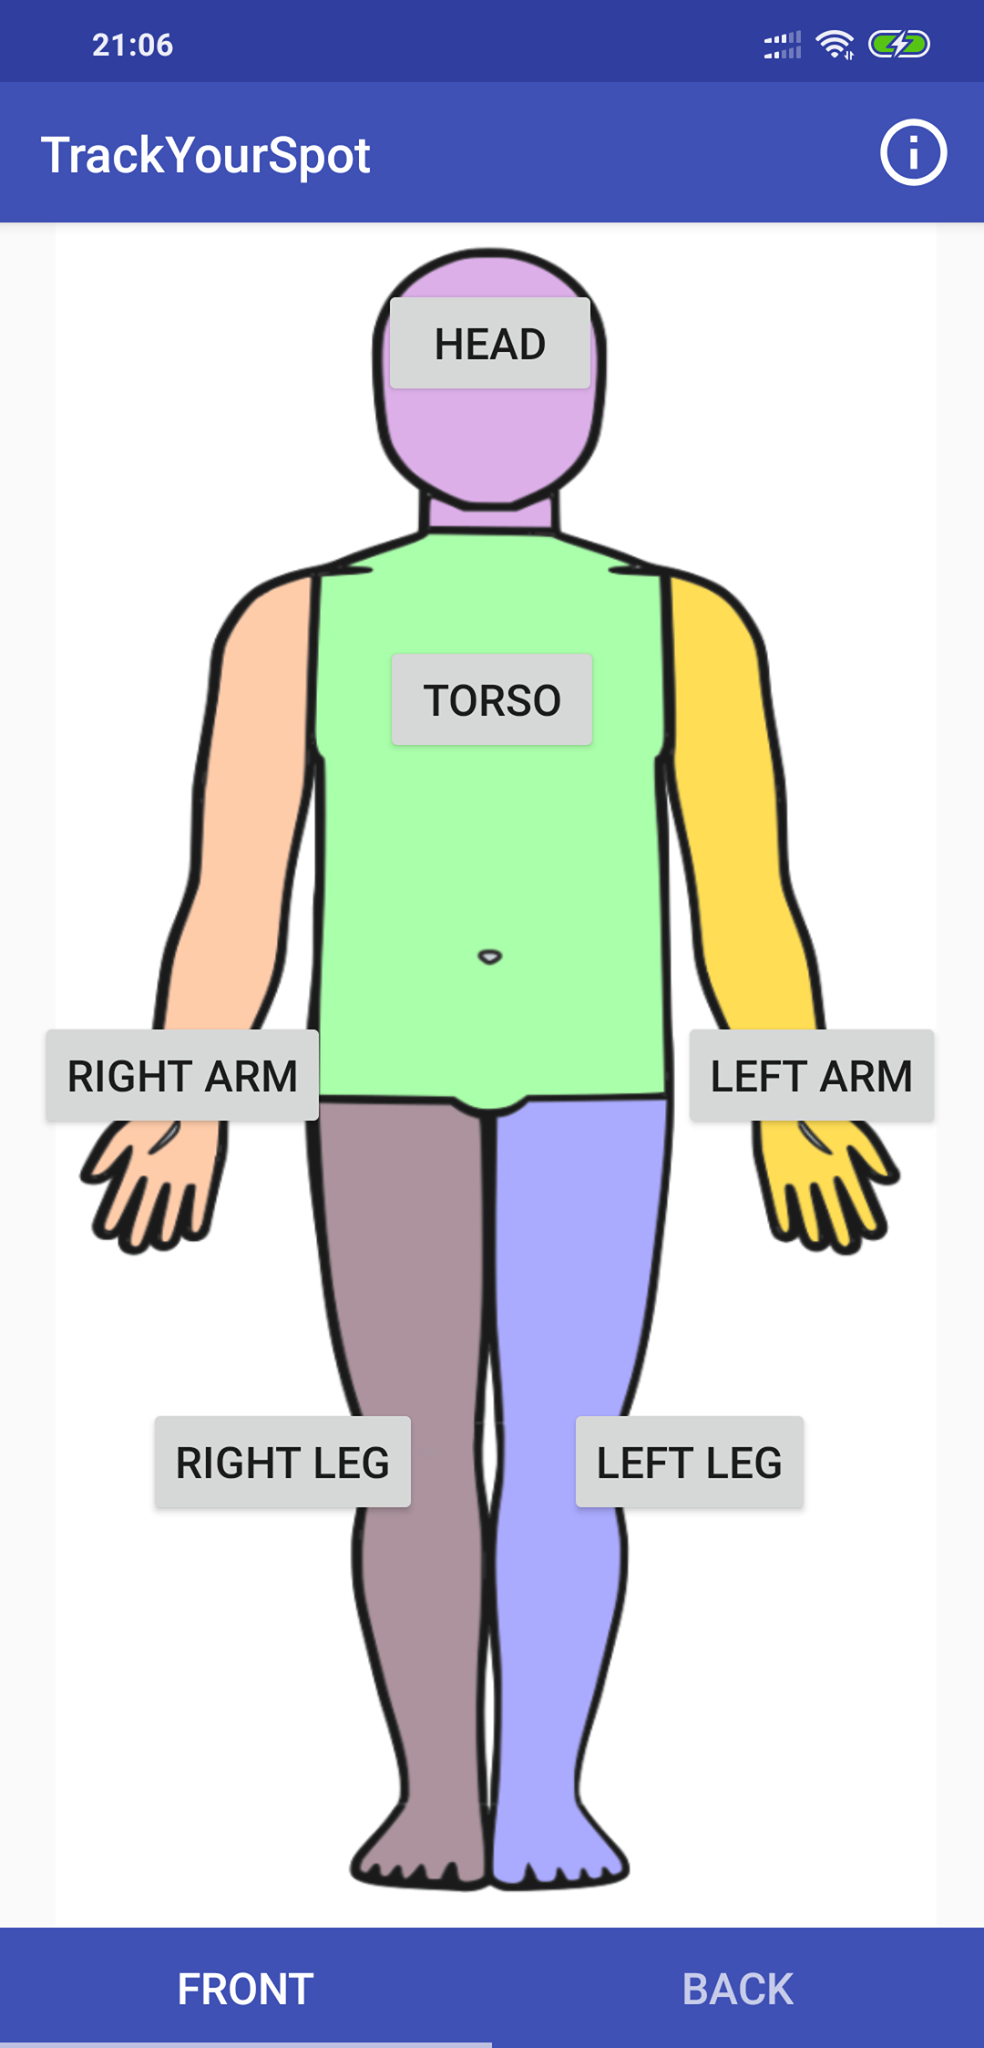
\includegraphics[height=10cm]{figures/frontbodybuttons.png}
        \caption{Front Body Screen}
    \end{subfigure}%
    ~
    \begin{subfigure}[t]{0.5\textwidth}
        \centering
        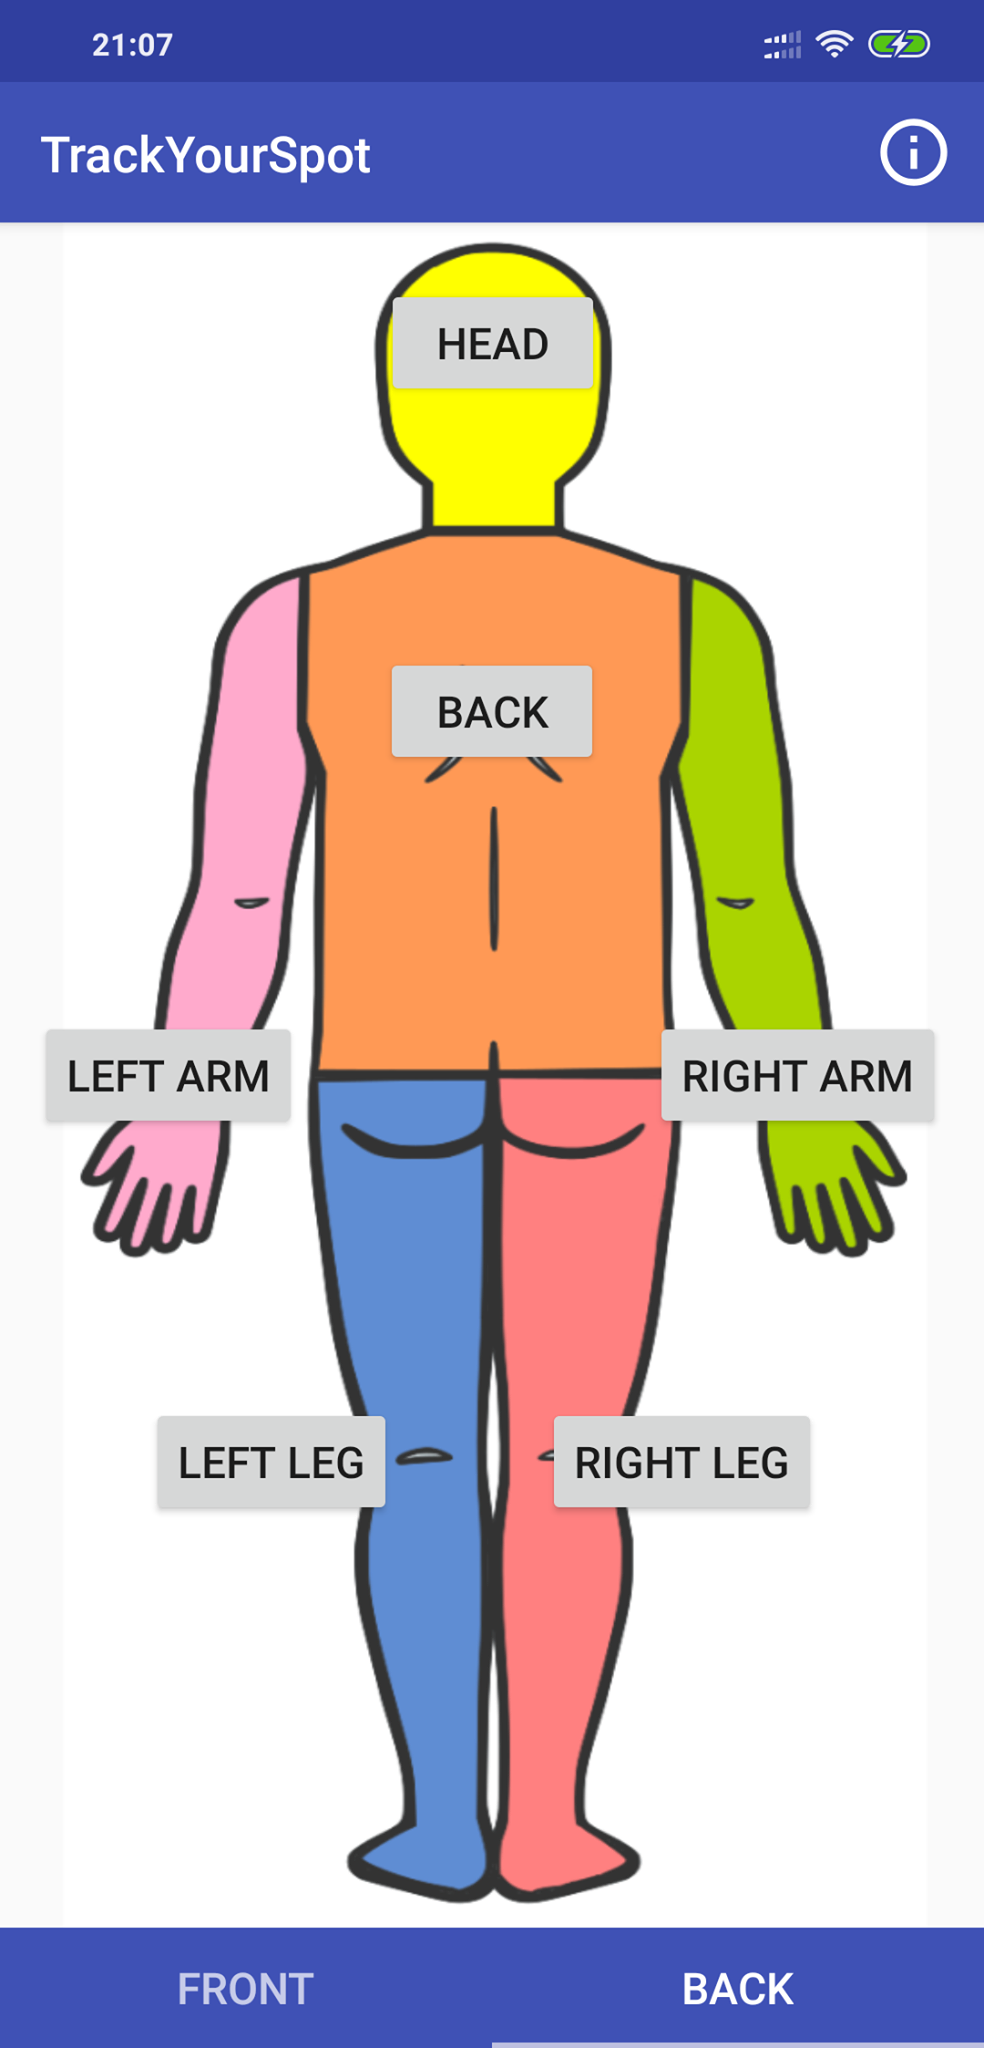
\includegraphics[height=10cm]{figures/backbodybuttons.png}
        \caption{Back Body Screen}
    \end{subfigure}
    \caption{App homepage body screen}
    \label{fig:bodyfinalscreen}
\end{figure*}

\clearpage
\begin{figure*}[t!]
    \centering
    \begin{subfigure}[t]{0.5\textwidth}
        \centering
        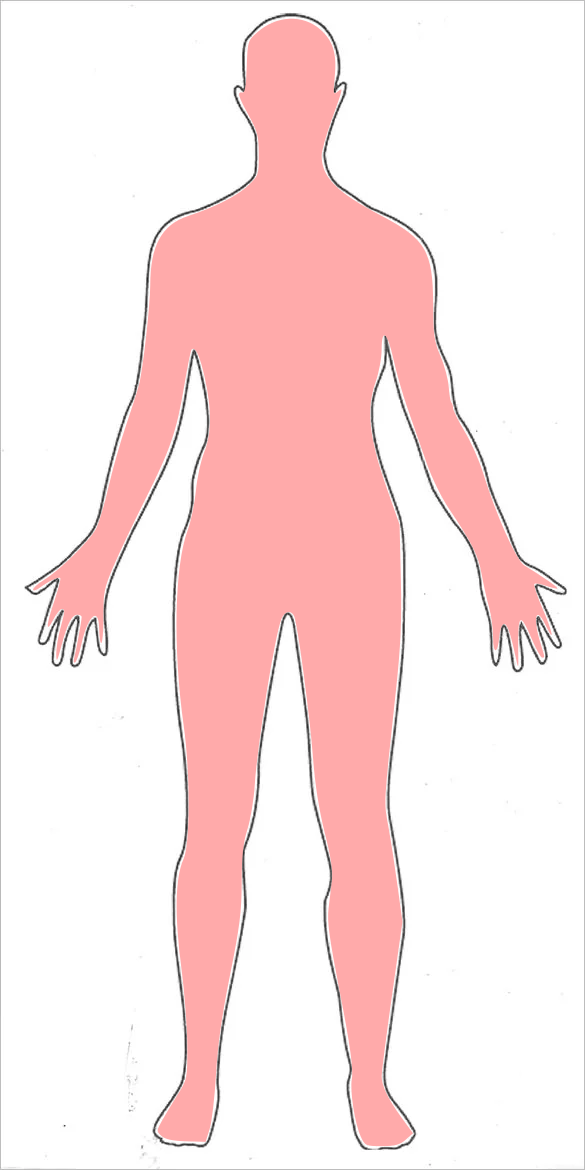
\includegraphics[height=10cm]{figures/bodydesign1front.png}
    \end{subfigure}%
    ~
    \begin{subfigure}[t]{0.5\textwidth}
        \centering
        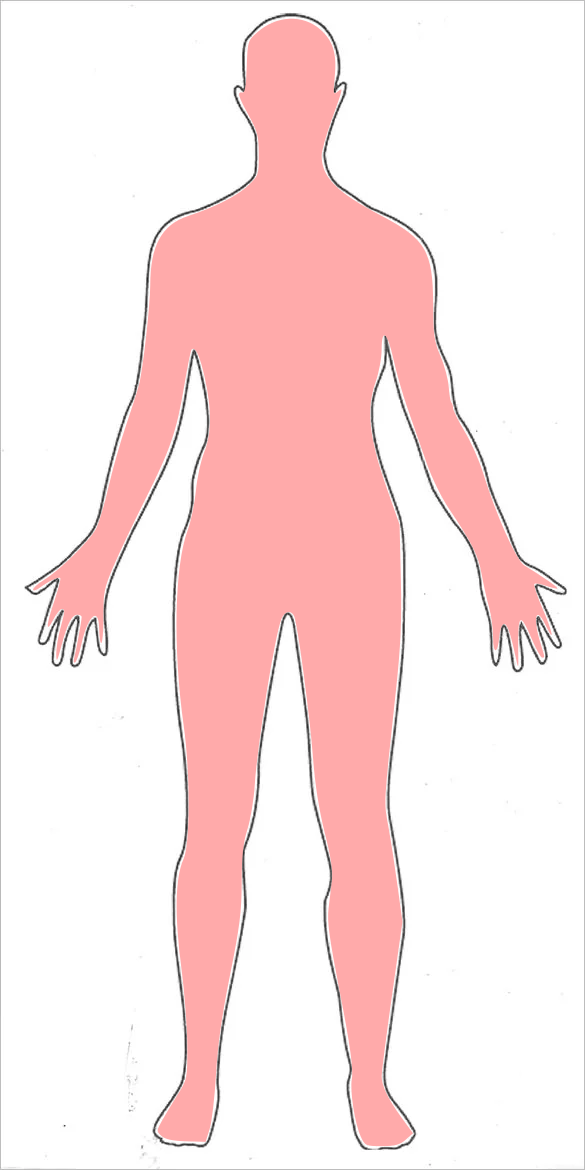
\includegraphics[height=10cm]{figures/bodydesign1front.png}
    \end{subfigure}
    \caption{Iteration 1 Body Designs}
    \label{fig:it1design}
\end{figure*}

\begin{figure*}[t!]
    \centering
    \begin{subfigure}[t]{0.5\textwidth}
        \centering
        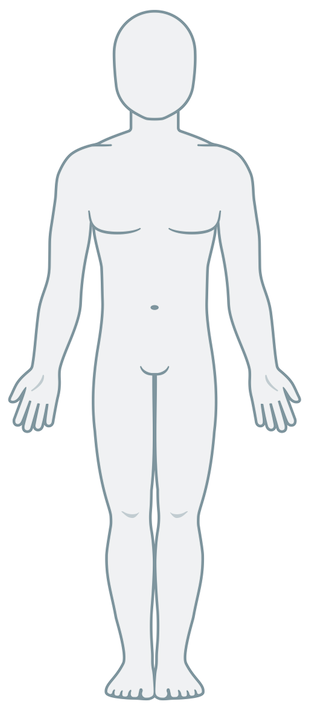
\includegraphics[height=10cm]{figures/bodydesign2front.png}
    \end{subfigure}%
    ~
    \begin{subfigure}[t]{0.5\textwidth}
        \centering
        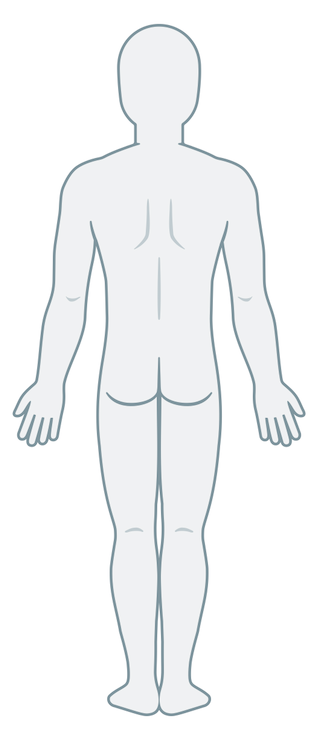
\includegraphics[height=10cm]{figures/bodydesign2back.png}
    \end{subfigure}
    \caption{Iteration 2 Body Designs}
    \label{fig:it2design}
\end{figure*}

\clearpage
\begin{figure*}[t!]
    \centering
    \begin{subfigure}[t]{0.5\textwidth}
        \centering
        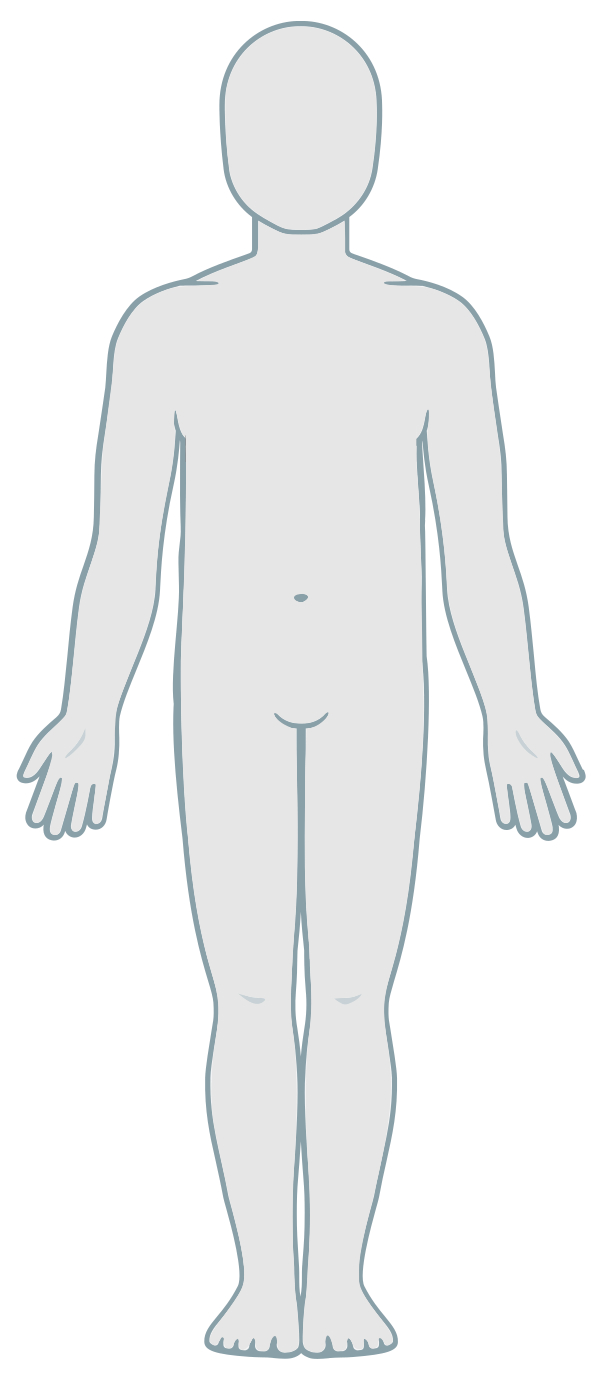
\includegraphics[height=10cm]{figures/bodydesign3front.jpg}
    \end{subfigure}%
    ~
    \begin{subfigure}[t]{0.5\textwidth}
        \centering
        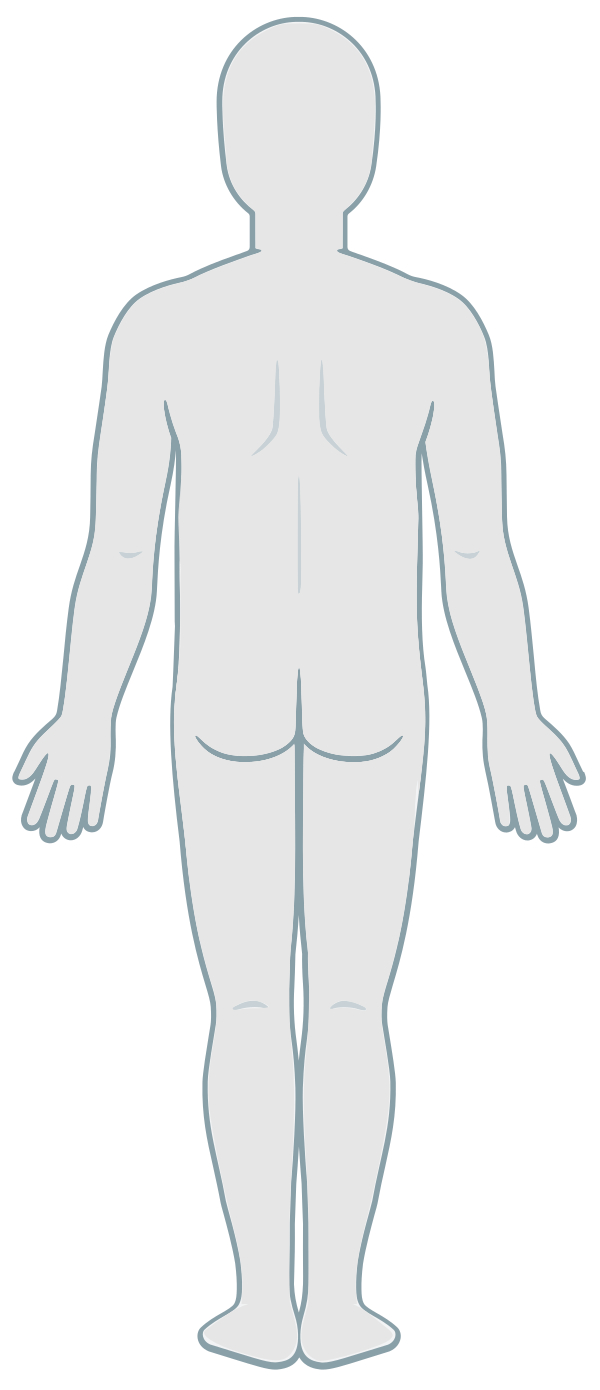
\includegraphics[height=10cm]{figures/bodydesign3back.jpg}
    \end{subfigure}
    \caption{Iteration 3 Body Designs}
    \label{fig:it3design}
\end{figure*}

\begin{figure*}[t!]
    \centering
    \begin{subfigure}[t]{0.5\textwidth}
        \centering
        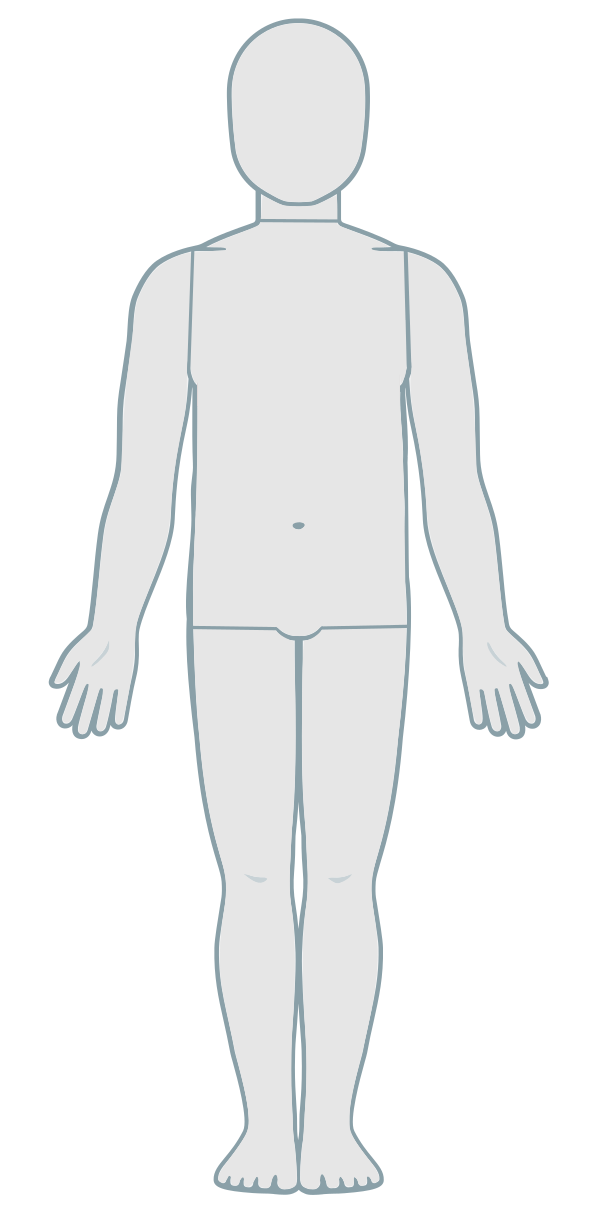
\includegraphics[height=10cm]{figures/bodydesign4front.png}
    \end{subfigure}%
    ~
    \begin{subfigure}[t]{0.5\textwidth}
        \centering
        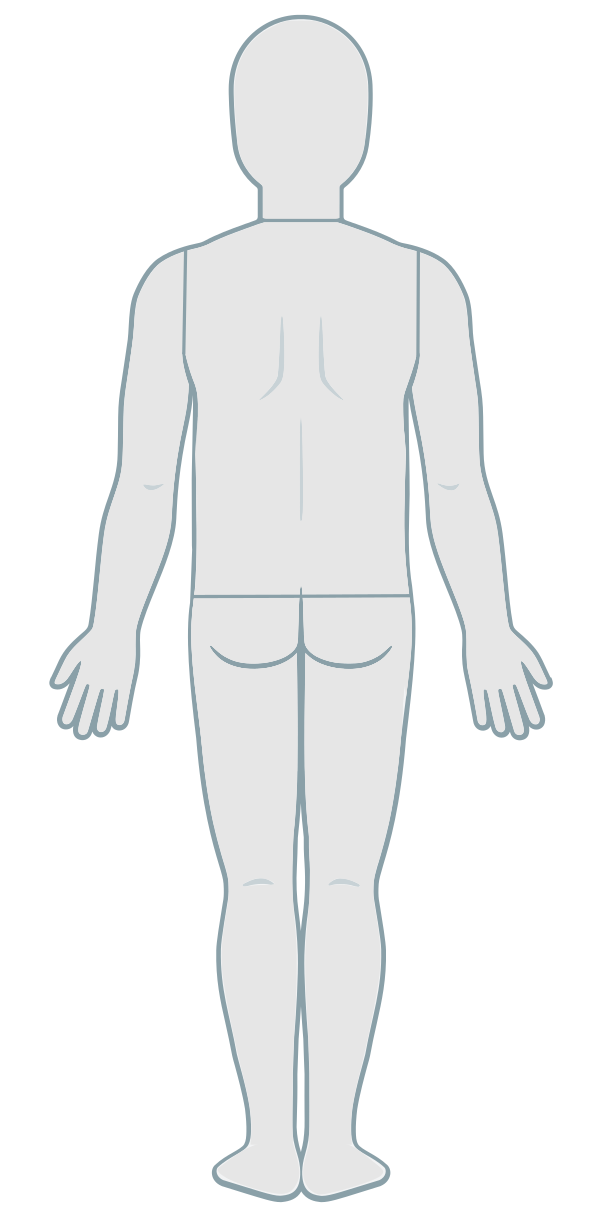
\includegraphics[height=10cm]{figures/bodydesign4back.png}
    \end{subfigure}
    \caption{Iteration 4 Body Designs}
    \label{fig:it4design}
\end{figure*}

\clearpage
\begin{figure*}[t!]
    \centering
    \begin{subfigure}[t]{0.5\textwidth}
        \centering
        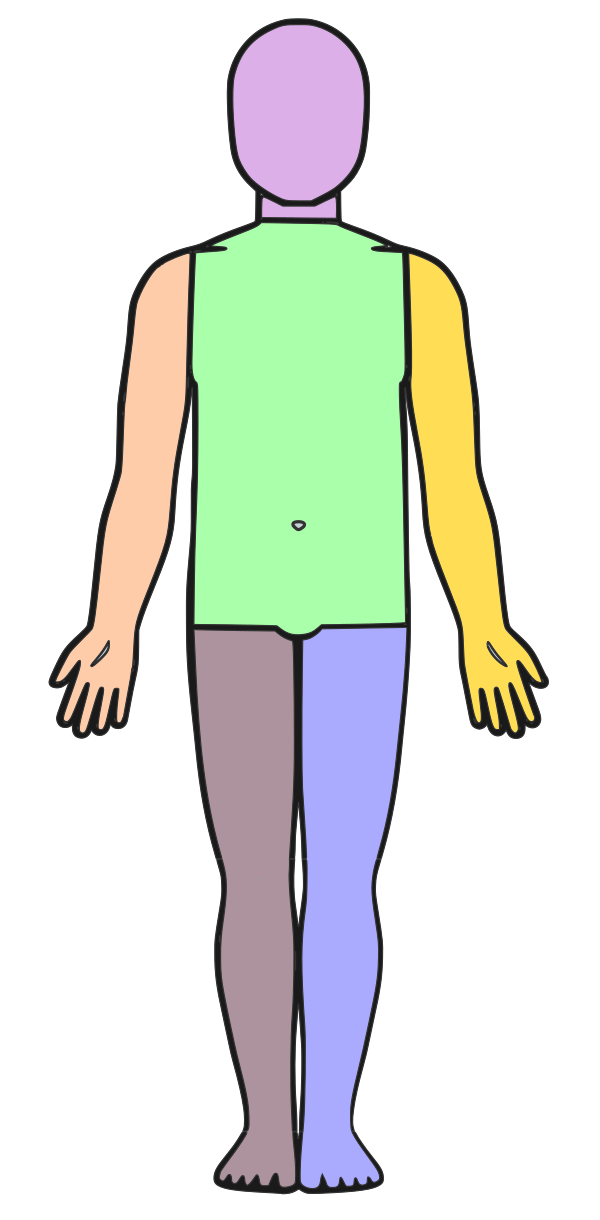
\includegraphics[height=10cm]{figures/bodydesign5front.png}
    \end{subfigure}%
    ~
    \begin{subfigure}[t]{0.5\textwidth}
        \centering
        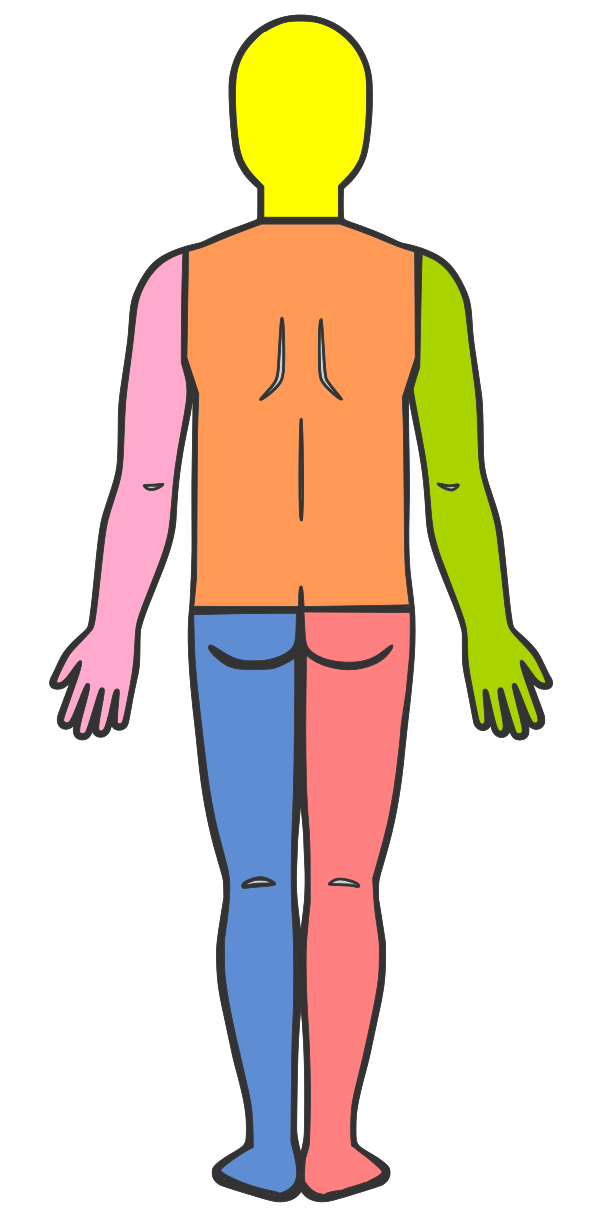
\includegraphics[height=10cm]{figures/bodydesign5back.png}
    \end{subfigure}
    \caption{Iteration 5 Body Designs}
    \label{fig:it15design}
\end{figure*}




\subsection{Information Screens} \label{sec:infoscreens}
As the title suggests, the information screens provide some background information on how to use the app in a safe manner. The screens in question are displayed in figure \ref{fig:infoscreens}. In order, the screens provide the following information concerning the following points:
\begin{enumerate}
    \item Danger of Skin Cancer
    \item Changes in Appeareance
    \item Preventing Skin Cancer
    \item Consulting a Doctor
\end{enumerate}

Ideally, the tutorial would also contain guidance on operating within the app, however, this would go against material design guidelines \cite{onboarding}, which suggest keeping tutorial screens short. A well-designed app user interface should require minimal tutorial help for the app to be used.

\clearpage
\begin{figure*}[t!]
    \centering
    \begin{subfigure}[t]{0.5\textwidth}
        \centering
        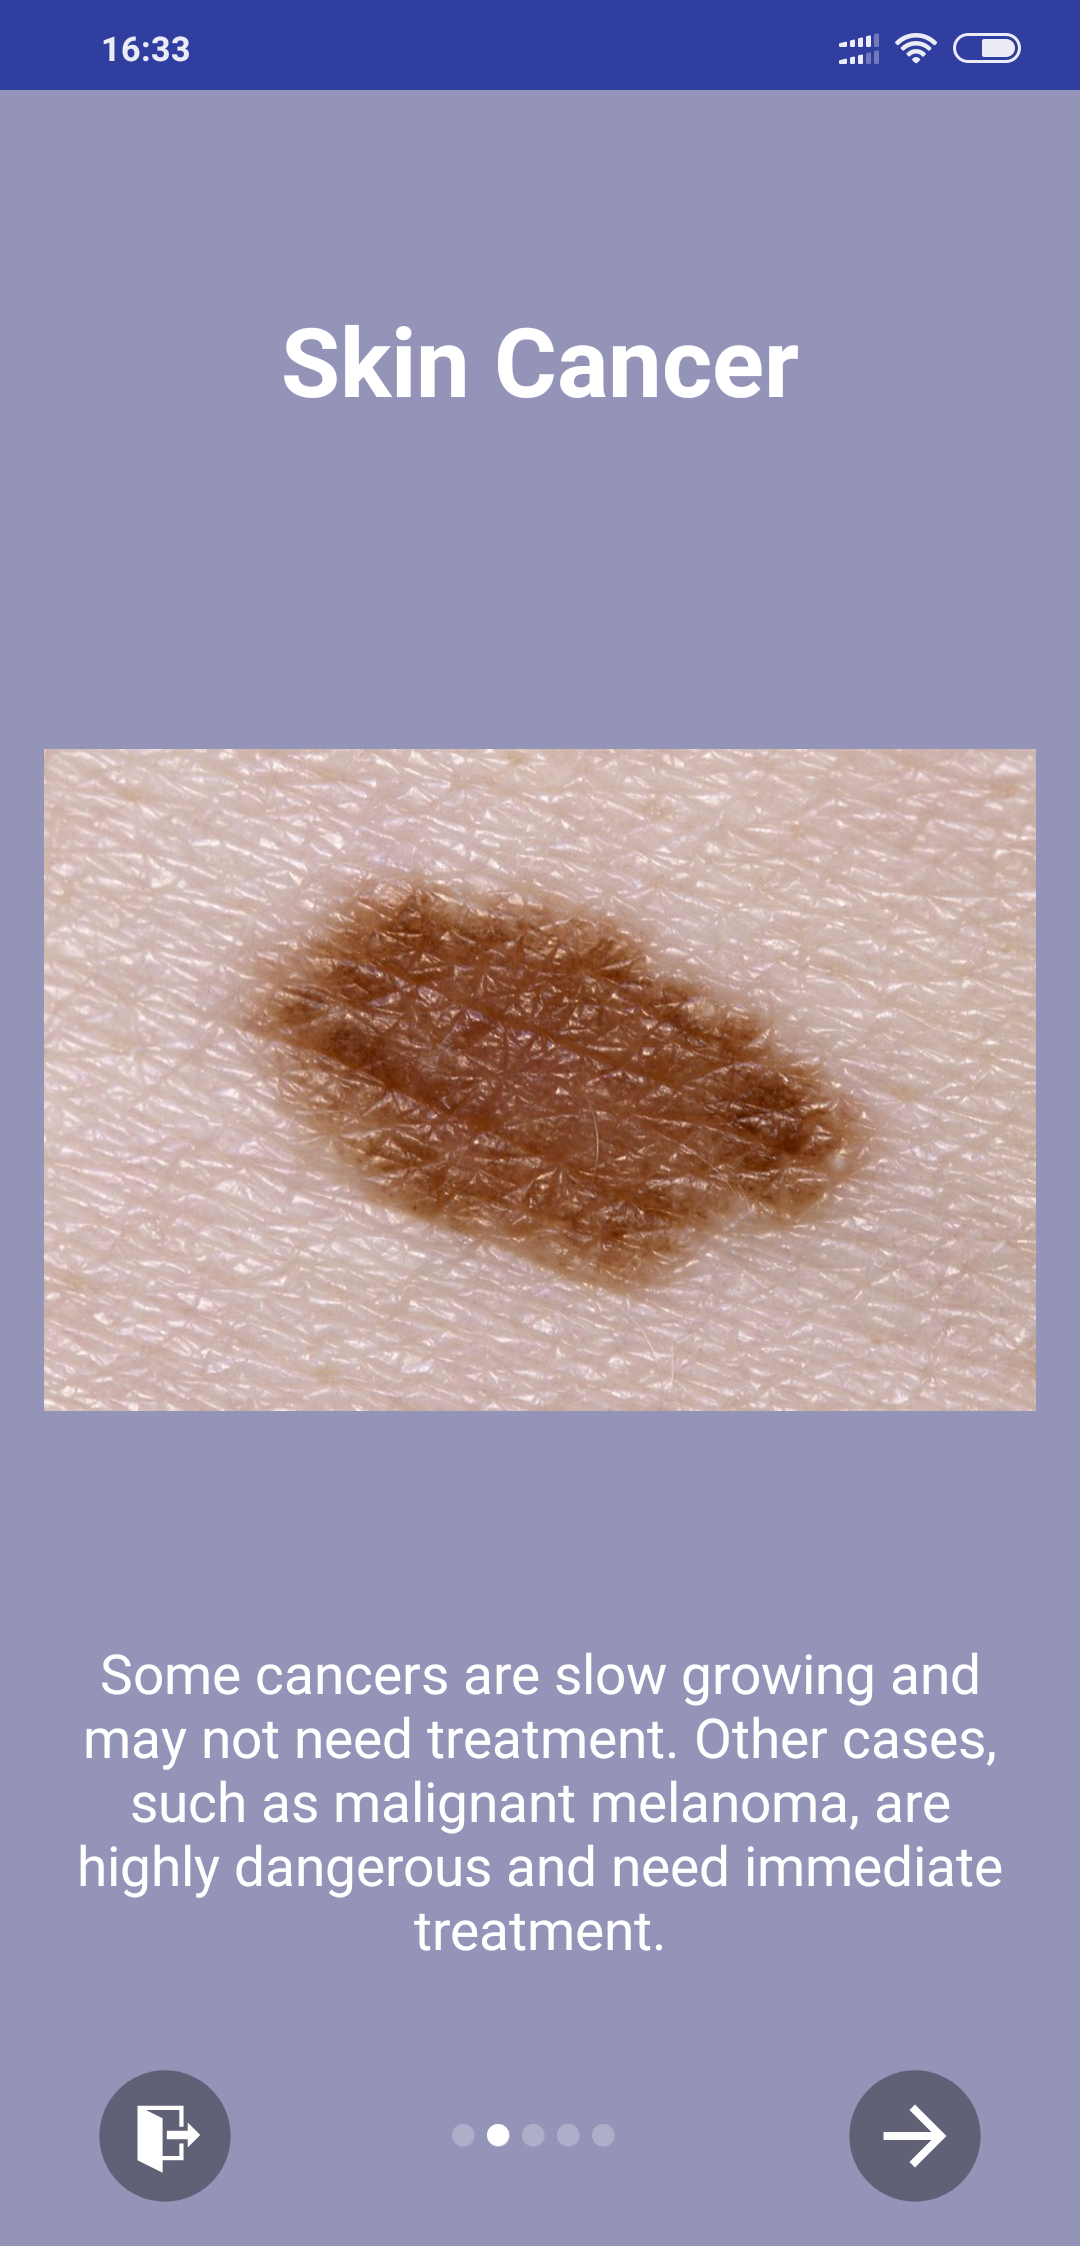
\includegraphics[height=10cm]{figures/info1_android.png}
        \caption{}
    \end{subfigure}%
    ~
    \begin{subfigure}[t]{0.5\textwidth}
        \centering
        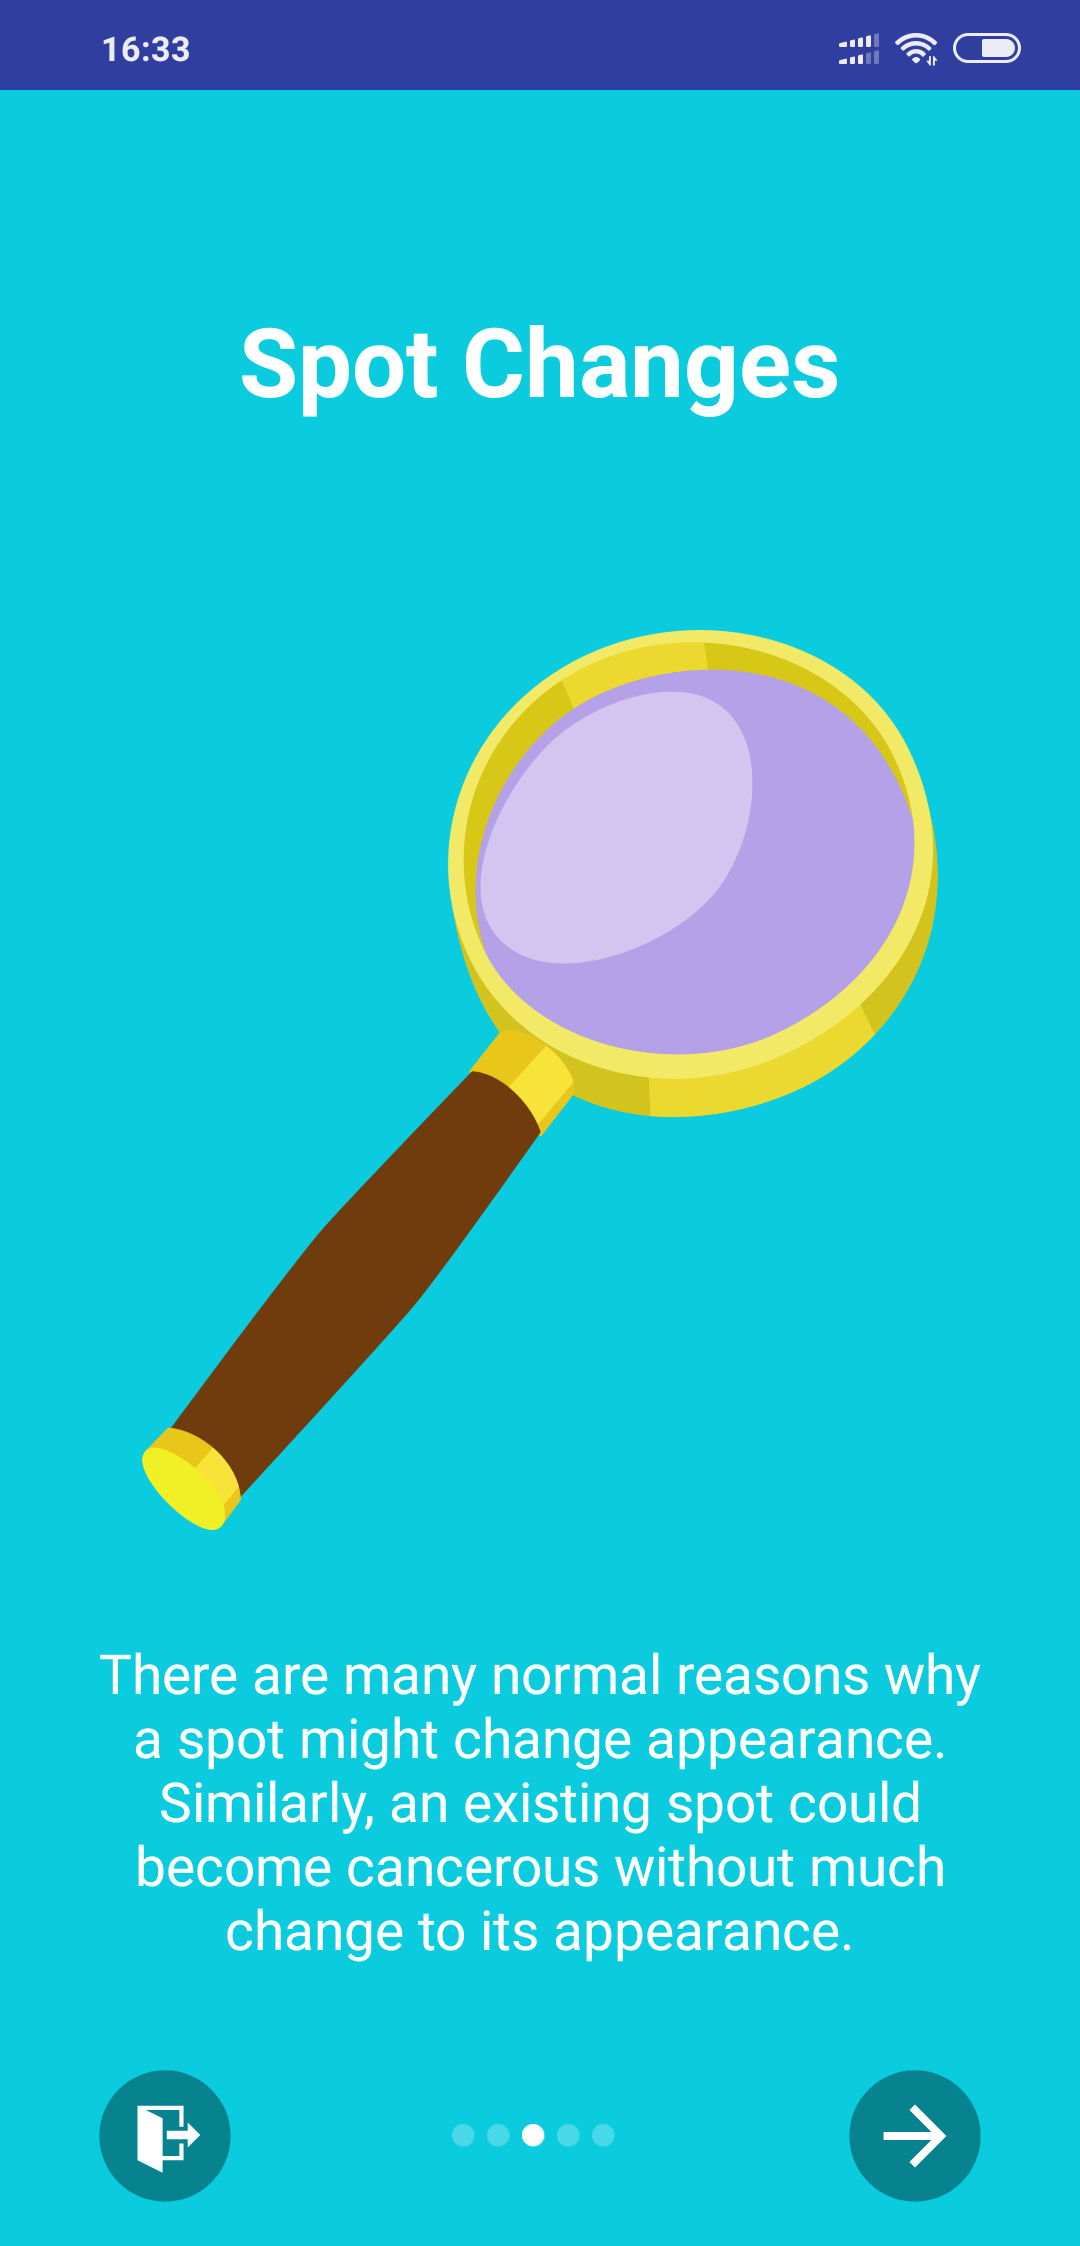
\includegraphics[height=10cm]{figures/info2_android.png}
        \caption{}
    \end{subfigure}
    \begin{subfigure}[t]{0.5\textwidth}
        \centering
        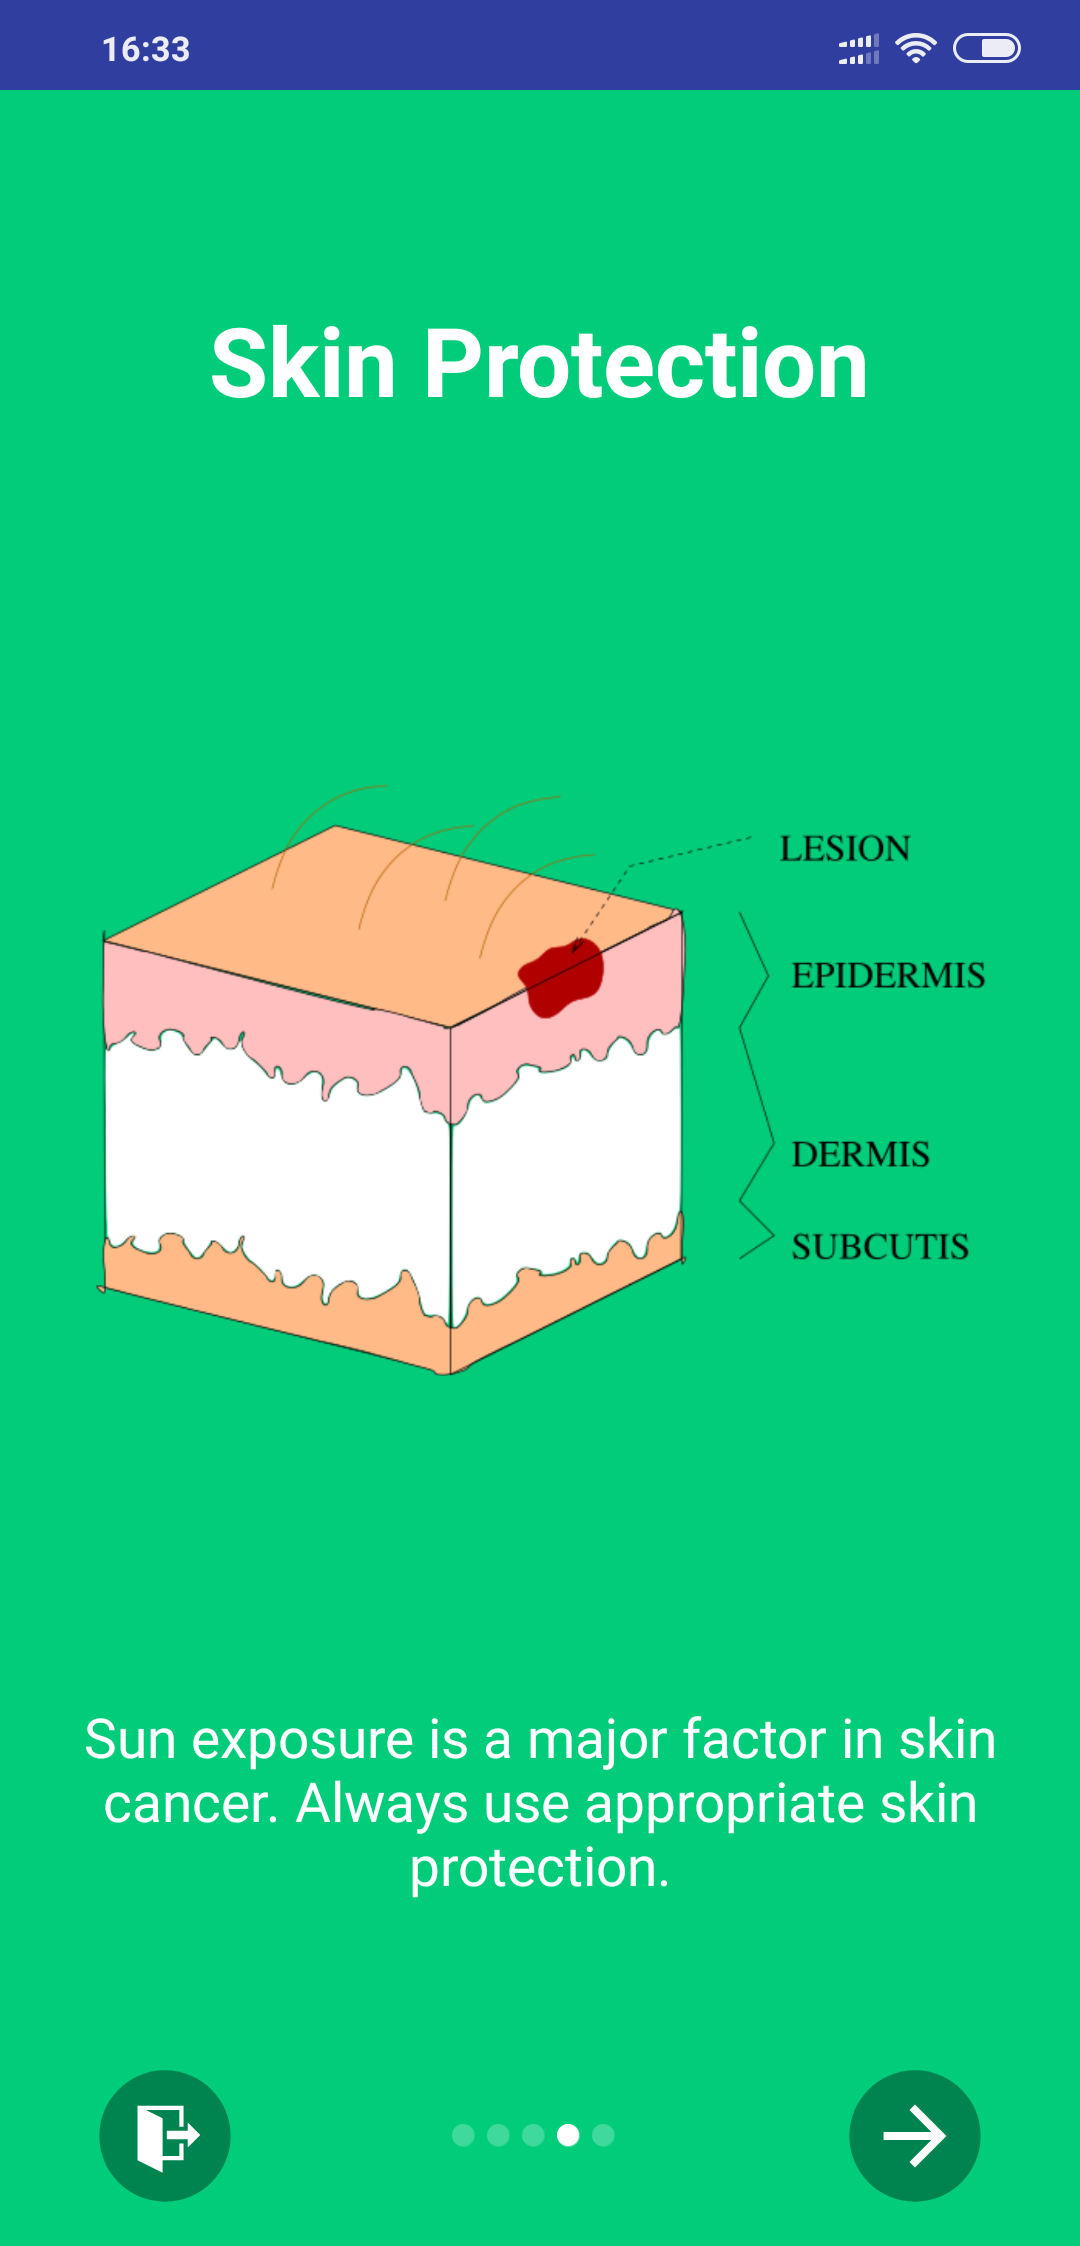
\includegraphics[height=10cm]{figures/info3_android.png}
        \caption{}
    \end{subfigure}%
    ~
    \begin{subfigure}[t]{0.5\textwidth}
        \centering
        
\includegraphics[height=10cm]{figures/info4_android.png}
        \caption{}
    \end{subfigure}
    \caption{Providing background information to the user through Information Screens}
    \label{fig:infoscreens}
\end{figure*}

\subsection{Old Spot Screen} \label{sec:oldspotscreen}
More accurately, this screen can be described as the screen displaying all previously added spots by the user in a selected body part. For example, if the user previously added the spots "Worrying Spot" and "Small normal spot" on their right arm, then these would be displayed in a list format on this screen. Each list item shows the spot name, a thumbnail of the spot, and the path of the spot in storage. From this screen, the user can:
\begin{itemize}
\item Add a new spot : By pressing the "+" button on the top right corner of the screen
\item Open a previously added spot: By selecting the spot from the displayed list of spots
\item Return to the body screen: By pressing the "$\leftarrow$" arrow button on the top left corner of the screen
\end{itemize}

\begin{figure*}[t!]
    \centering
    \begin{subfigure}[t]{0.5\textwidth}
        \centering
        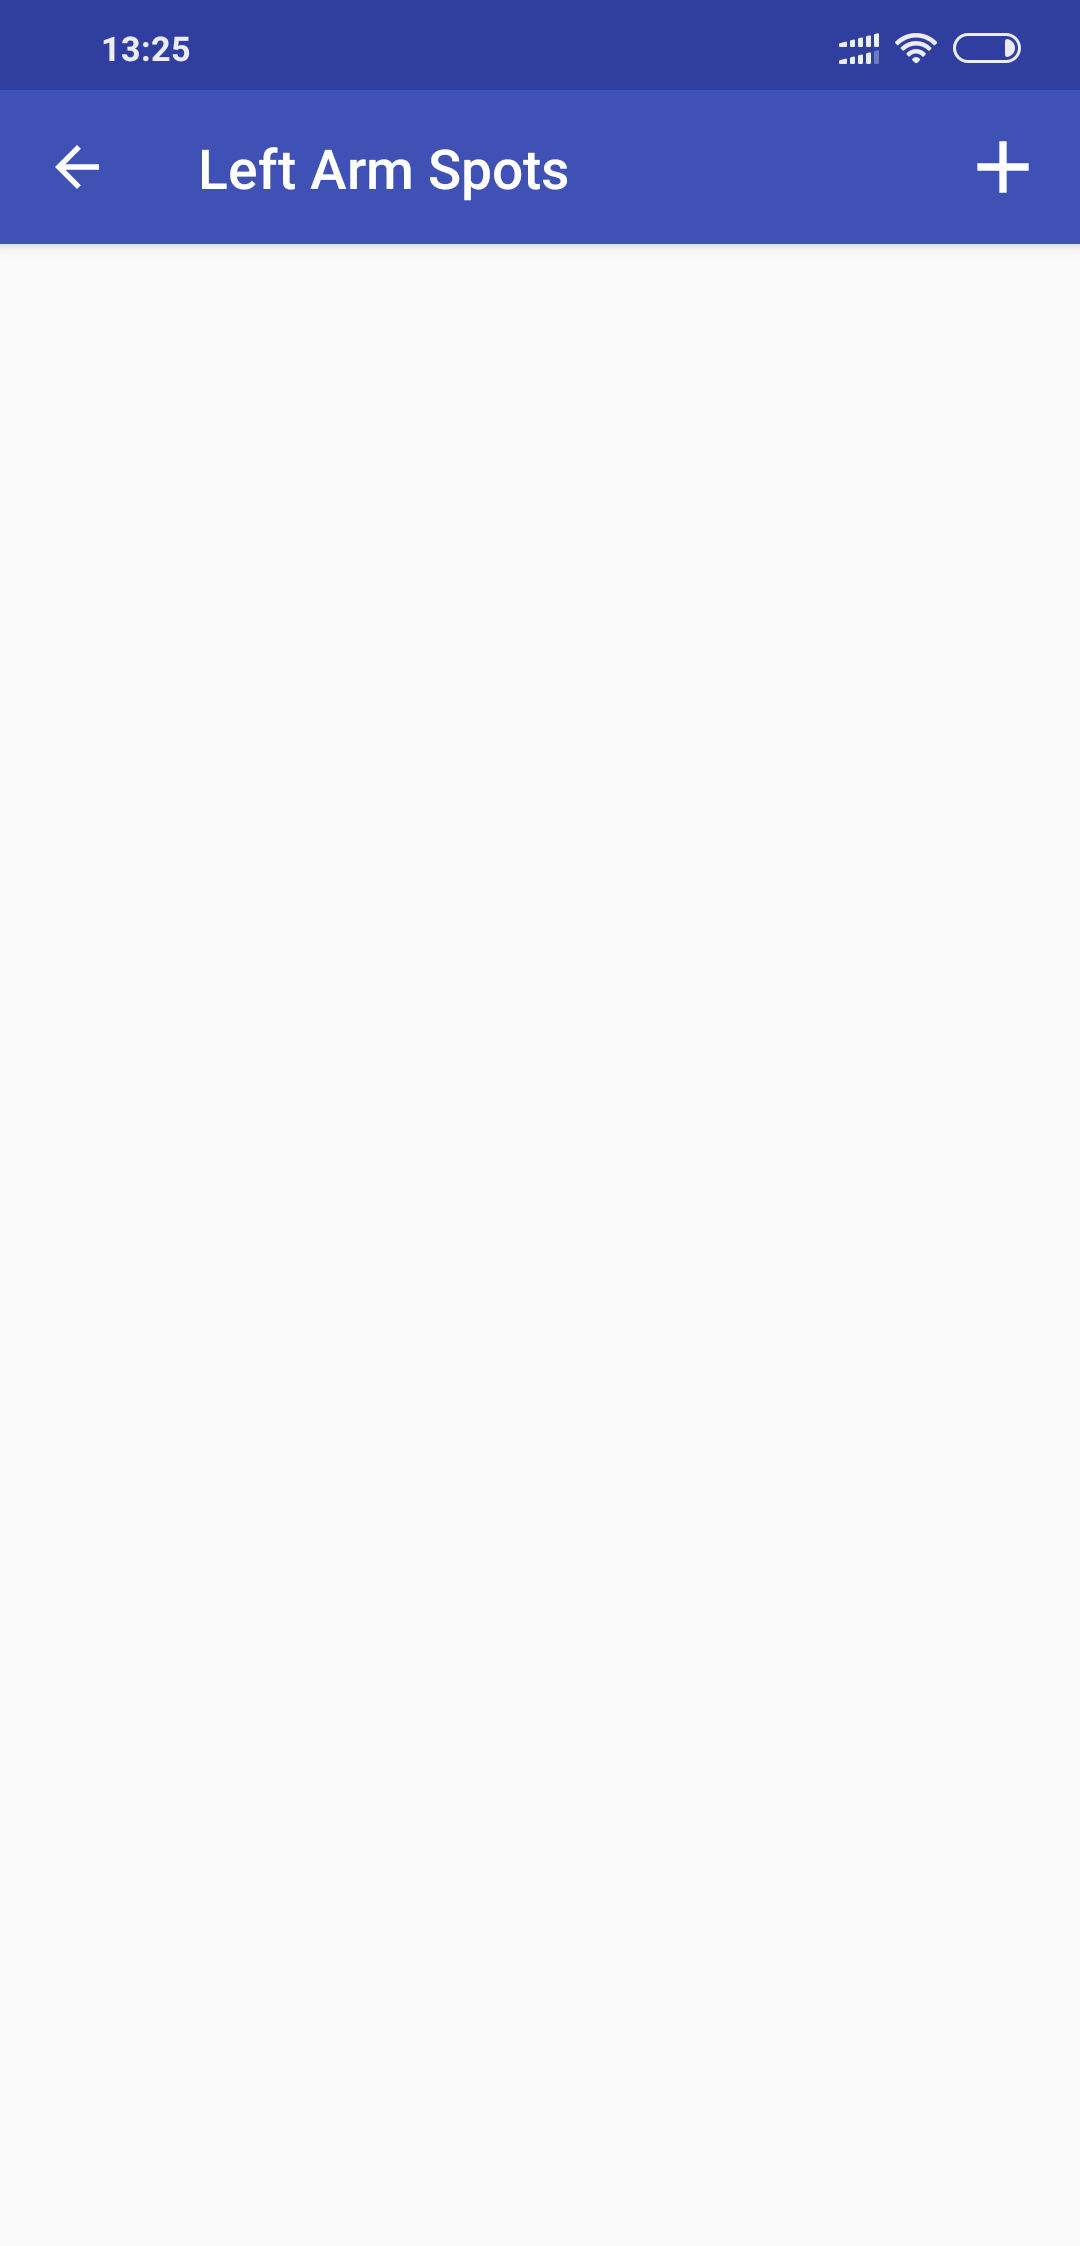
\includegraphics[height=10cm]{figures/spotlistempty_android.png}
        \caption{Empty Spot List}
    \end{subfigure}%
    ~
    \begin{subfigure}[t]{0.5\textwidth}
        \centering
        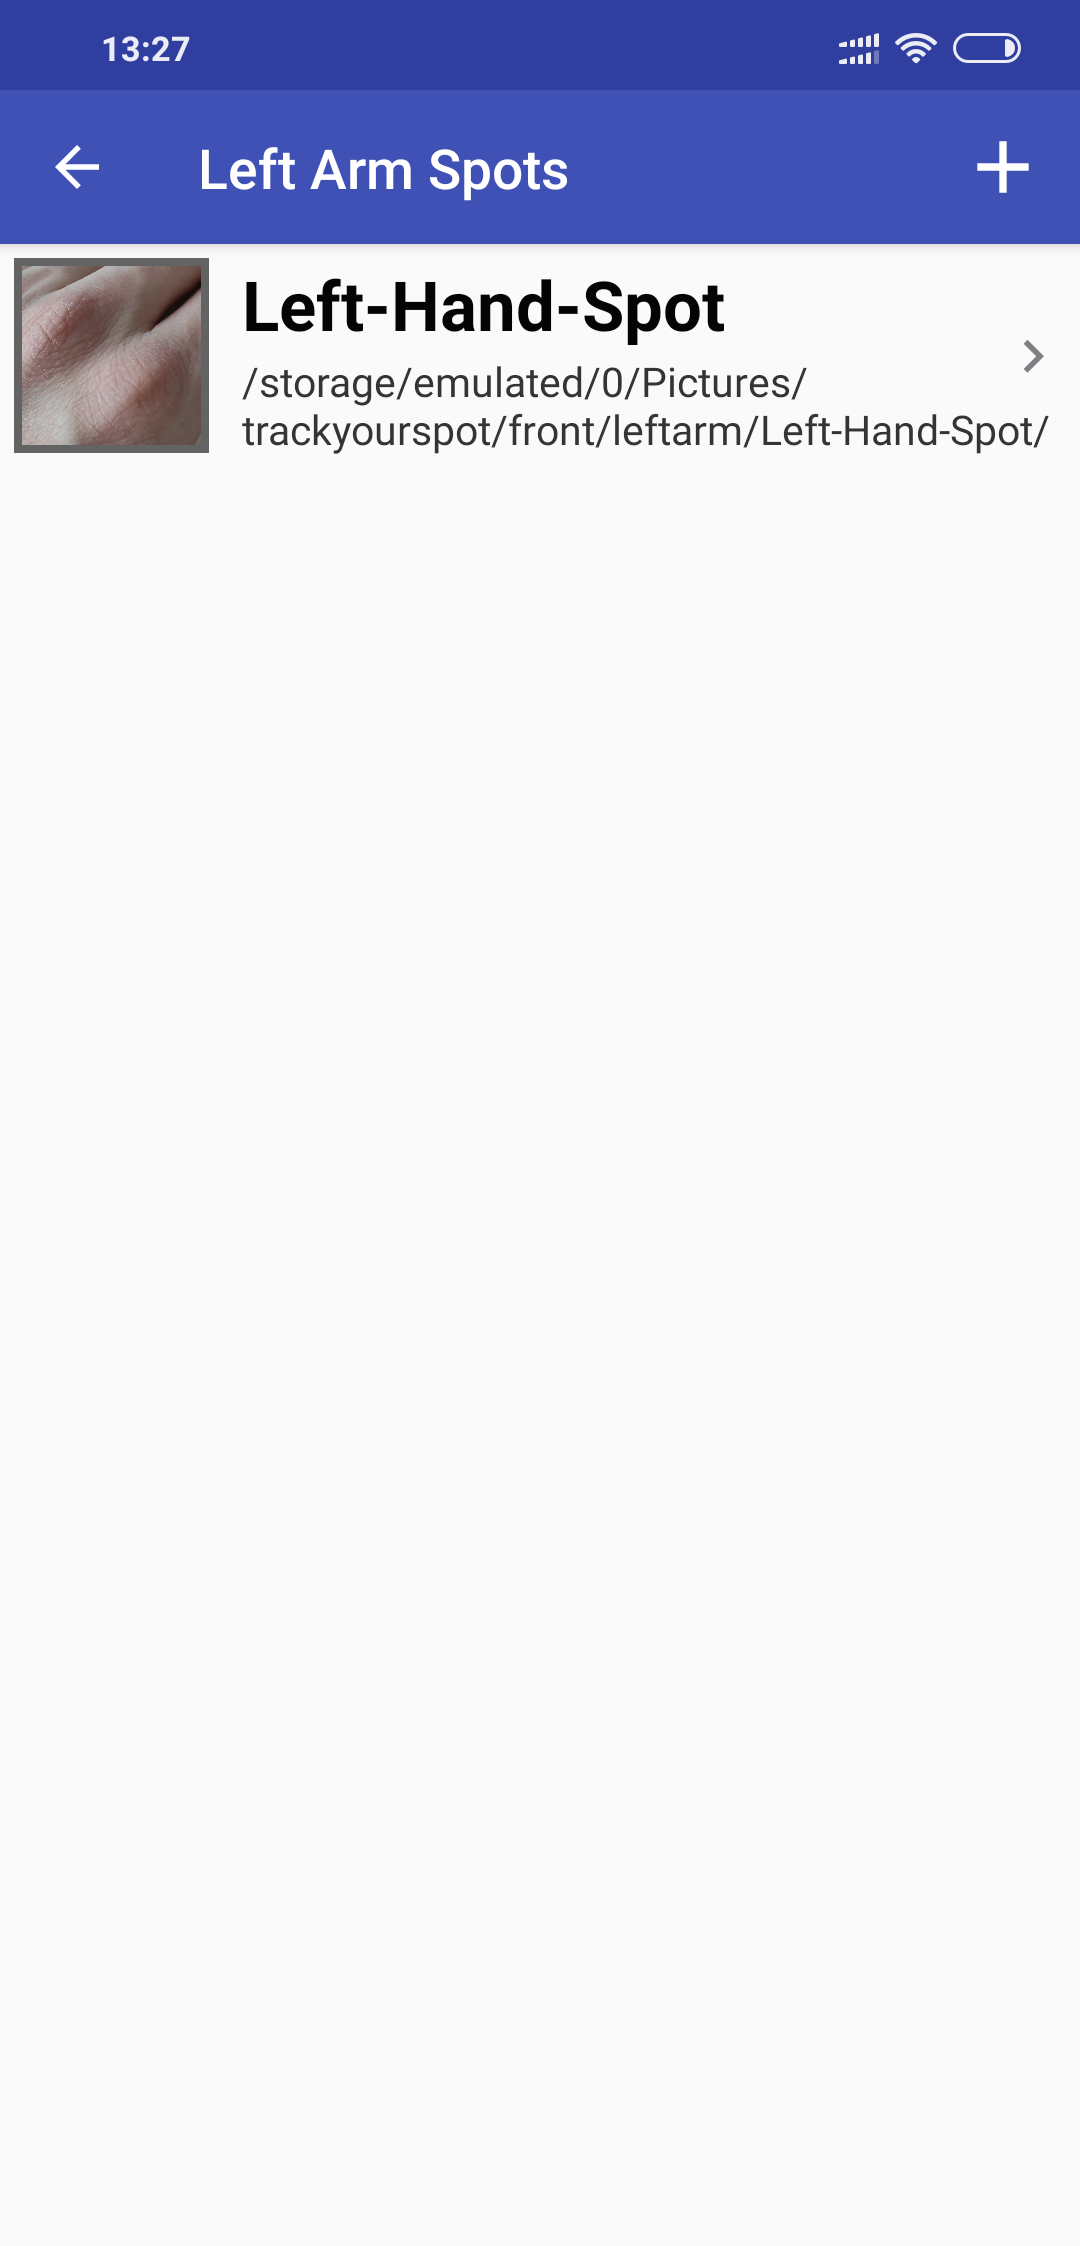
\includegraphics[height=10cm]{figures/spotlist_android.png}
        \caption{Left arm spot list after adding a spot}
    \end{subfigure}
    \caption{Old Spot Screen for the Left Arm}
\end{figure*}

\subsection{Camera and Cropping Screen}
These successive screens are displayed on two occasions: When a user elects to add a new spot, and when the user adds a new image to an old spot (spot update). This allows users to take a photo of a spot (Figure \ref{fig:cameraandcrop}), zoom in to a close up distance, and crop the image to a squared 1:1 aspect ratio. This ensures consistency across all images, so that all photos are of similar characteristics for easy comparison. The camera screen is provided by each user's default camera app, while the cropping screen is implemented through the uCrop Android Library \cite{yalantis_2019}. 

Using the Camera and uCrop API's means we are quite limited in customizing the appearance and design of these screens. The alternative would involve creating custom Activities and Screen layouts. However, this would require a very large amount of effort for a relatively low reward. Benefits would include drawing a "mask" or "frame" around the camera, so that the user knows how to better position the spot in the photo or cropping. This would also require implementing back-end storage manipulating functions for both the camera and cropping activities. On the contrary, using the APIs already provides a very flexible and user friendly UI, hence the decision was made to use these. 

Once the camera is open, the user can repeatedly take photos until they are happy with the image. This is indicated through the "\checkmark" or "x" symbols. Subsequently, the cropping activity opens the image. The cropping screen allows zooming in and rotating the image, both operated by a slider at the bottom of the screen. Once again, the user can proceed to save the photo with the "\checkmark" button, or cancel the action through the "x" button. This returns the app to the old spot or spot image list screens.

\begin{figure*}[t!]
    \centering
    \begin{subfigure}[t]{0.5\textwidth}
        \centering
        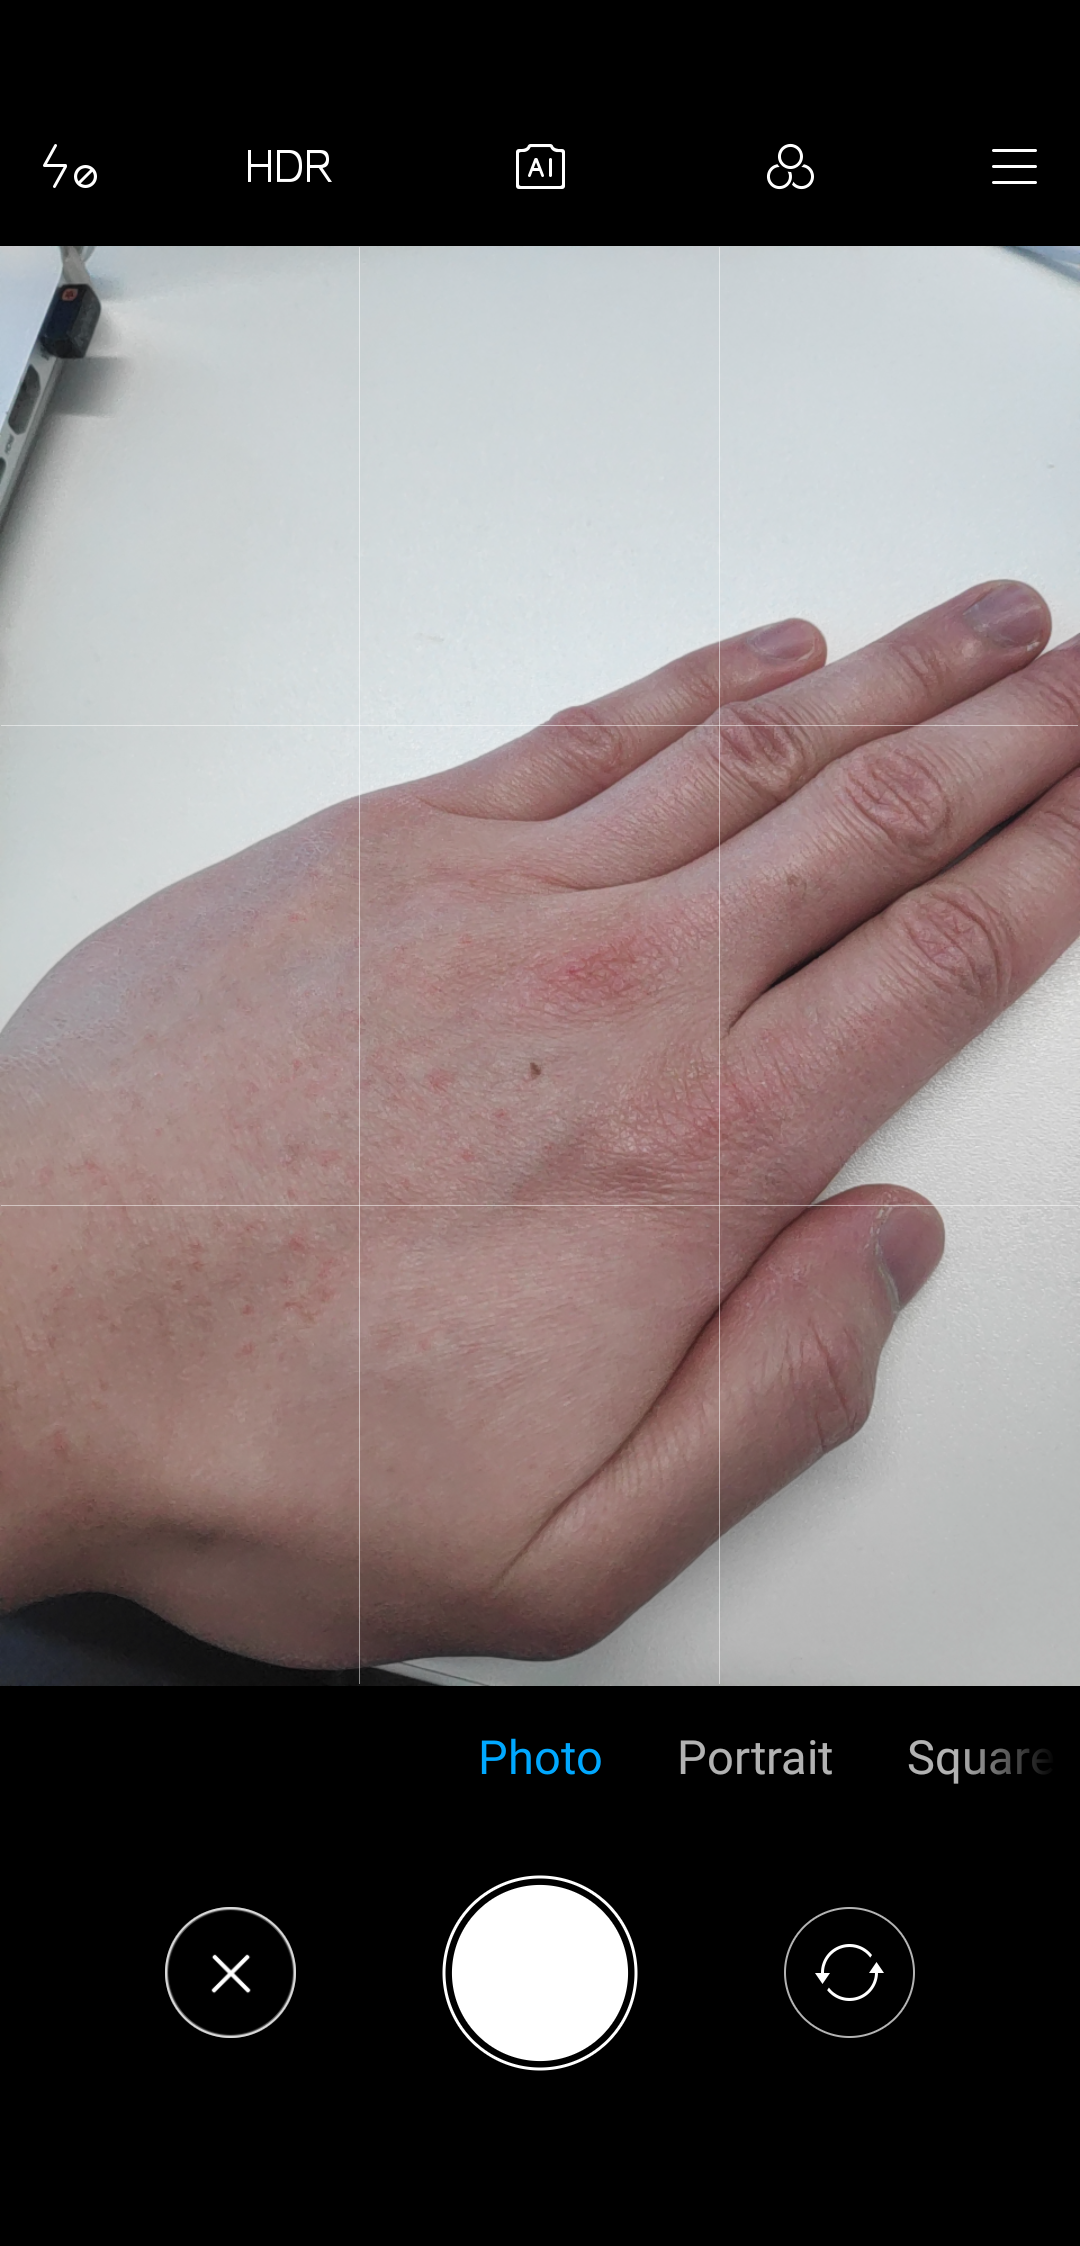
\includegraphics[height=10cm]{figures/camera1.png}
        \caption{Camera Screen after selecting to add a new spot}
    \end{subfigure}%
    ~
    \begin{subfigure}[t]{0.5\textwidth}
        \centering
        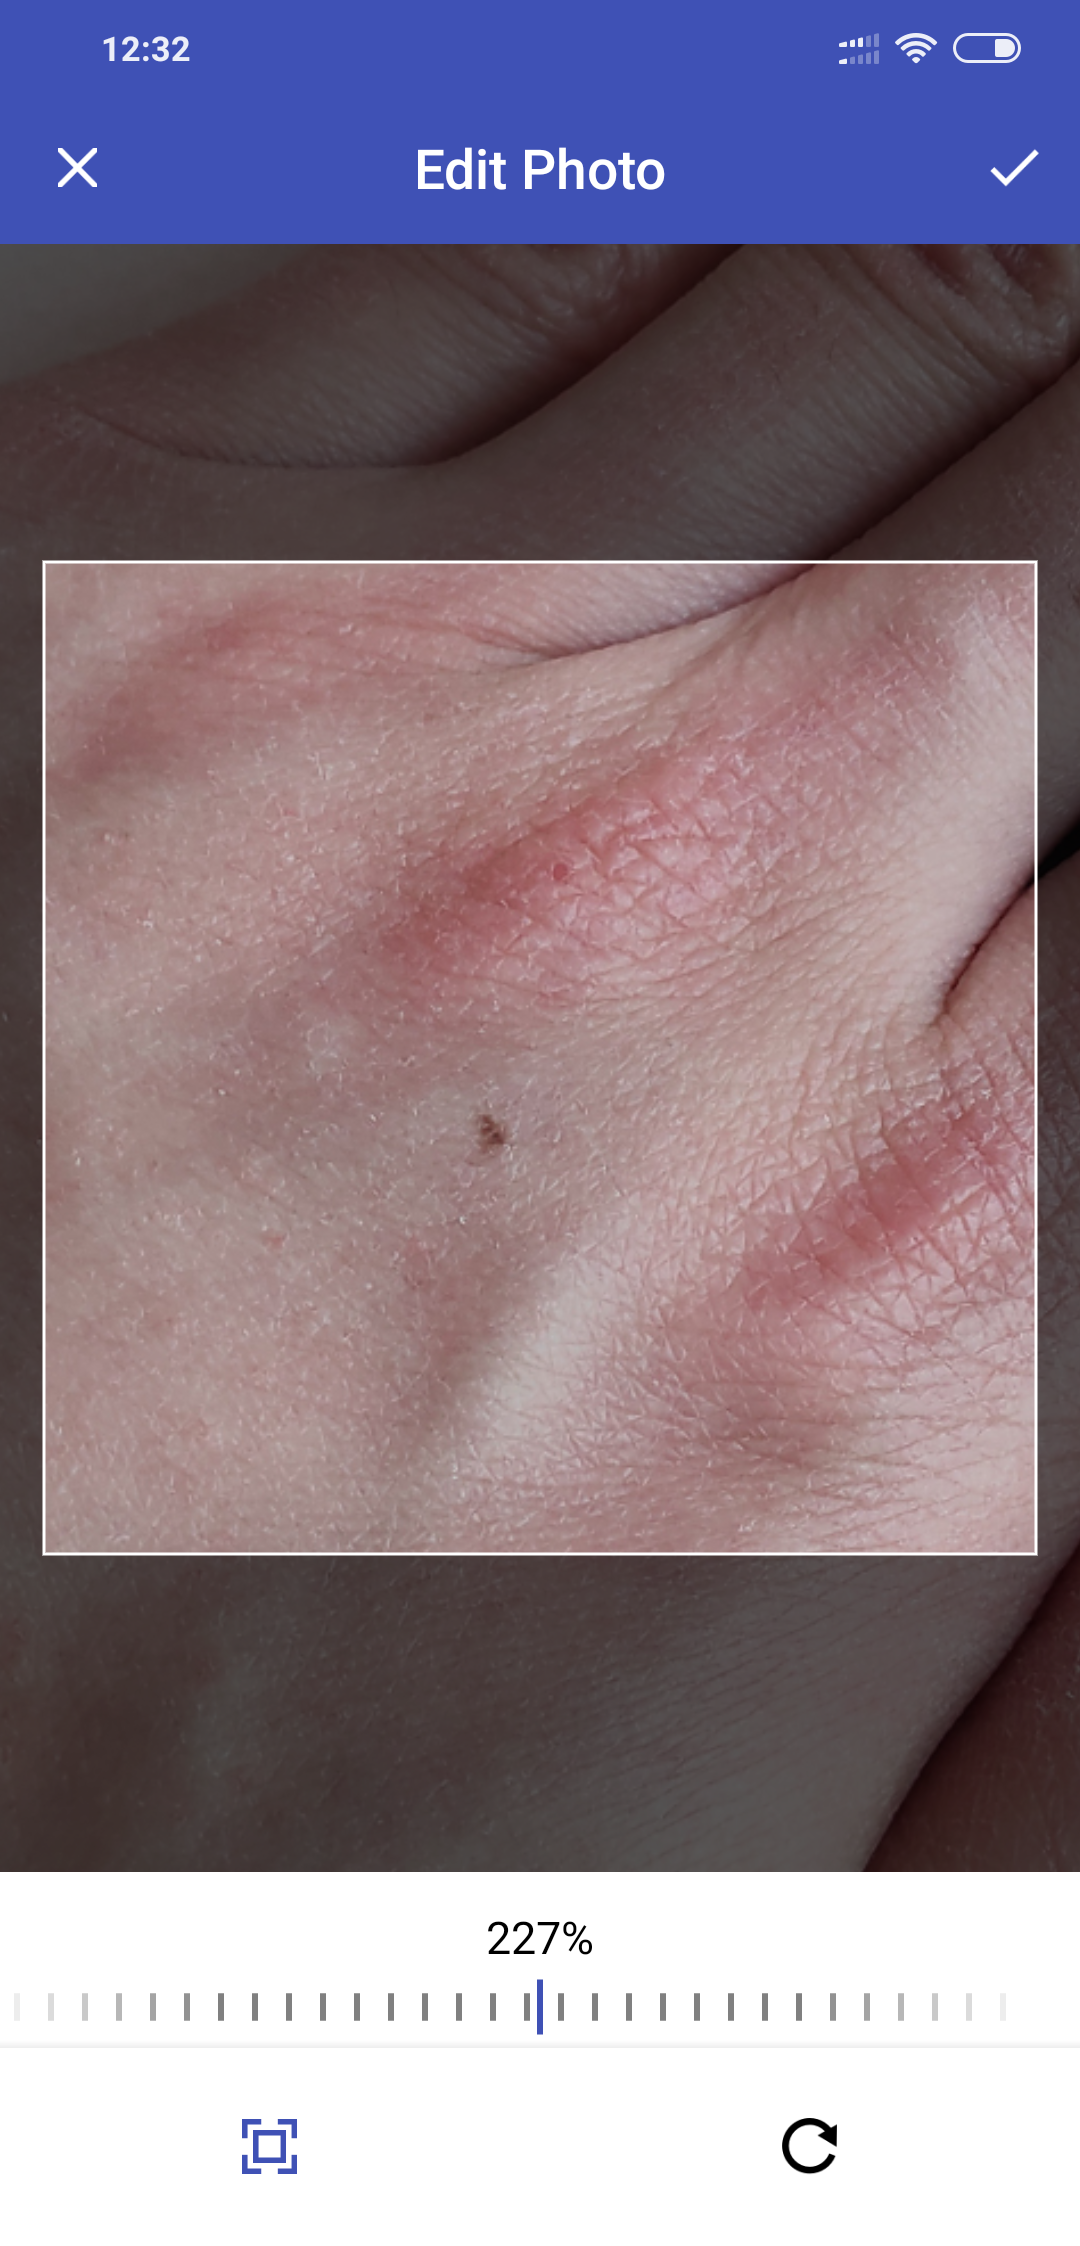
\includegraphics[height=10cm]{figures/crop1.png}
        \caption{Cropping Screen after zooming in to the chosen spot}
    \end{subfigure}
    \caption{Camera and Cropping Screens}
    \label{fig:cameraandcrop}
\end{figure*}

\subsection{Spot Naming Screen}
This screen is used to give a name to a new spot, this name is useful to better identify a spot when adding newer images in the future. Figures \ref{subfig:oldaddspot} and \ref{subfig:oldaddspotkeyboard} show the very first initial design, later evolving into designs \ref{subfig:newaddspotkeyboard} and \ref{subfig:newaddspotnokeyboard} (Showing and hiding the keyboard respectively).

This screen contains a text input field to name the spot, a large preview of the photo that has just been taken, and two aligned buttons labelled "Cancel" and "Confirm". Clicking either button would take the user back to the SpotList screen. However, the confirm button would succesfully add the new spot to the list, while the cancel button deletes the image and returns to the previous spot list.

To justify the final design, the advantages and disadvantages of both designs can be compared. The initial design appears to be very basic, lacking an option to cancel the process of adding the spot. The design makes little use of screen size, leaving much of the display blank and keeping the image preview small in size. This could prove to be an issue with tiny spots or low quality images. The new design in Figures \ref{subfig:newaddspotkeyboard} and \ref{subfig:newaddspotnokeyboard} addresses these issues accordingly, providing a much larger, half-screen view of the image, allowing even very small spots to be clearly visible (assuming the image has been cropped sensibly). The text entry field now has its own container, separating more clearly the different components of the screen. Following official Android design guidelines for image positioning \cite{materialdesignimageplacement}, the image has been anchored to the top of the screen, with text right below it, this also makes the app more consistent with common image or social networking apps. Furthermore, the image and name container will always be visible even with the keyboard displayed. Lastly, a "Cancel" button gives the user flexibility to restart the spot adding process if they are unhappy with the image. This can also be done with the "$\leftarrow$" arrow button on the top left corner.
\clearpage
\begin{figure*}[t!]
    \centering
    \begin{subfigure}[t]{0.5\textwidth}
        \centering
        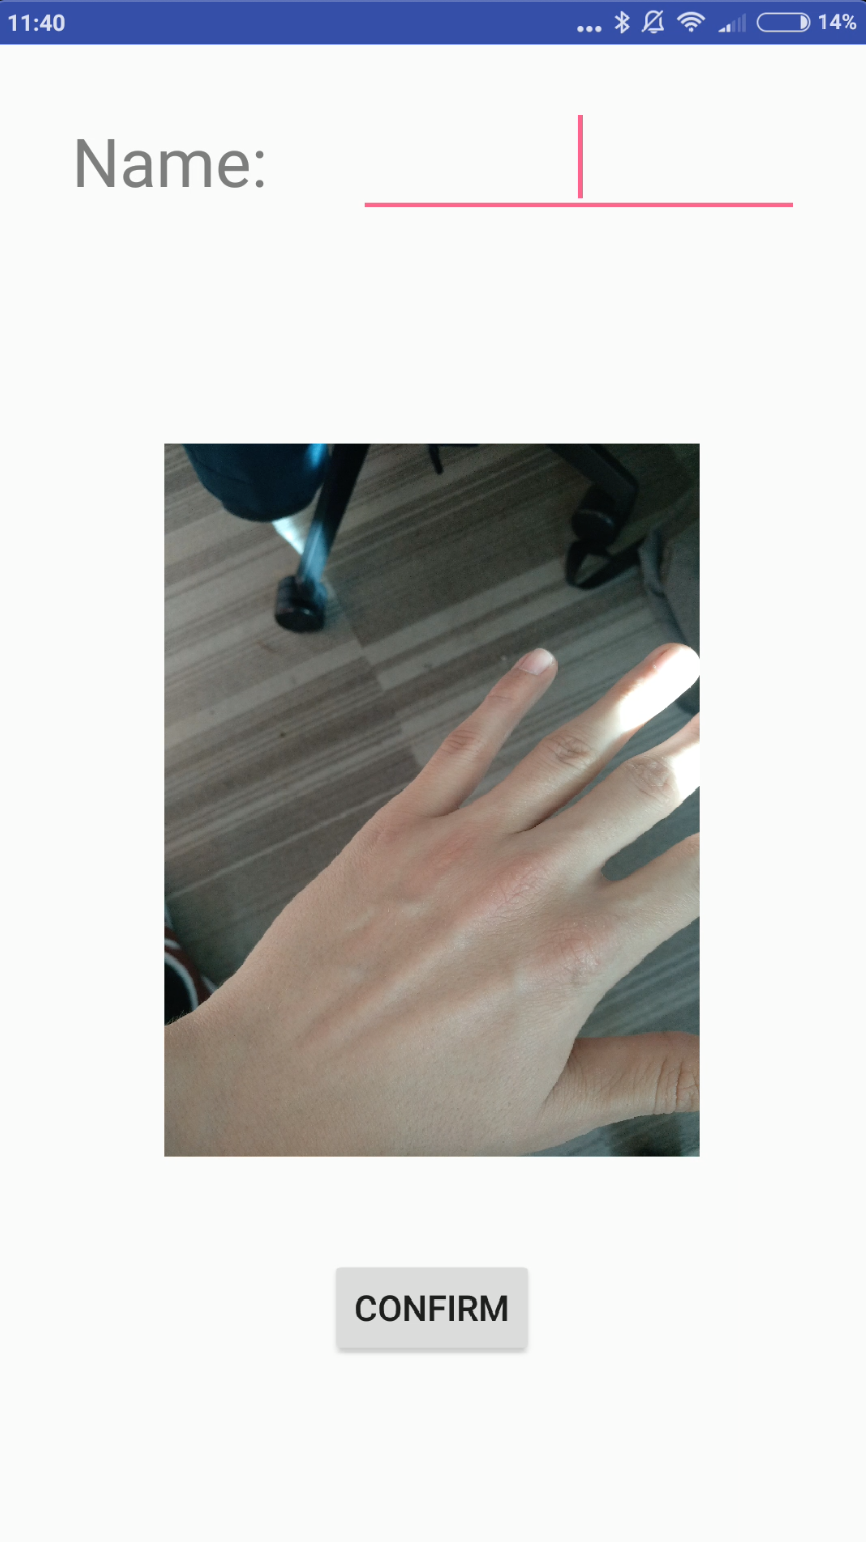
\includegraphics[height=10cm]{figures/addspot1.png}
        \caption{Initial AddSpot Activity screen}
        \label{subfig:oldaddspot}
    \end{subfigure}%
        ~
    \begin{subfigure}[t]{0.5\textwidth}
        \centering
        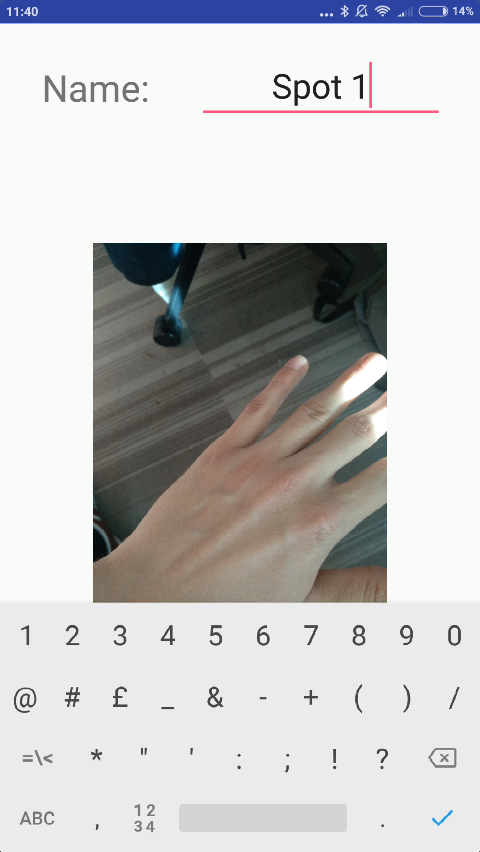
\includegraphics[height=10cm]{figures/oldaddspotkeyboard.png}
        \caption{Initial AddSpot Activity Screen showing the keyboard}
        \label{subfig:oldaddspotkeyboard}
    \end{subfigure}
    ~
    \begin{subfigure}[t]{0.5\textwidth}
        \centering
        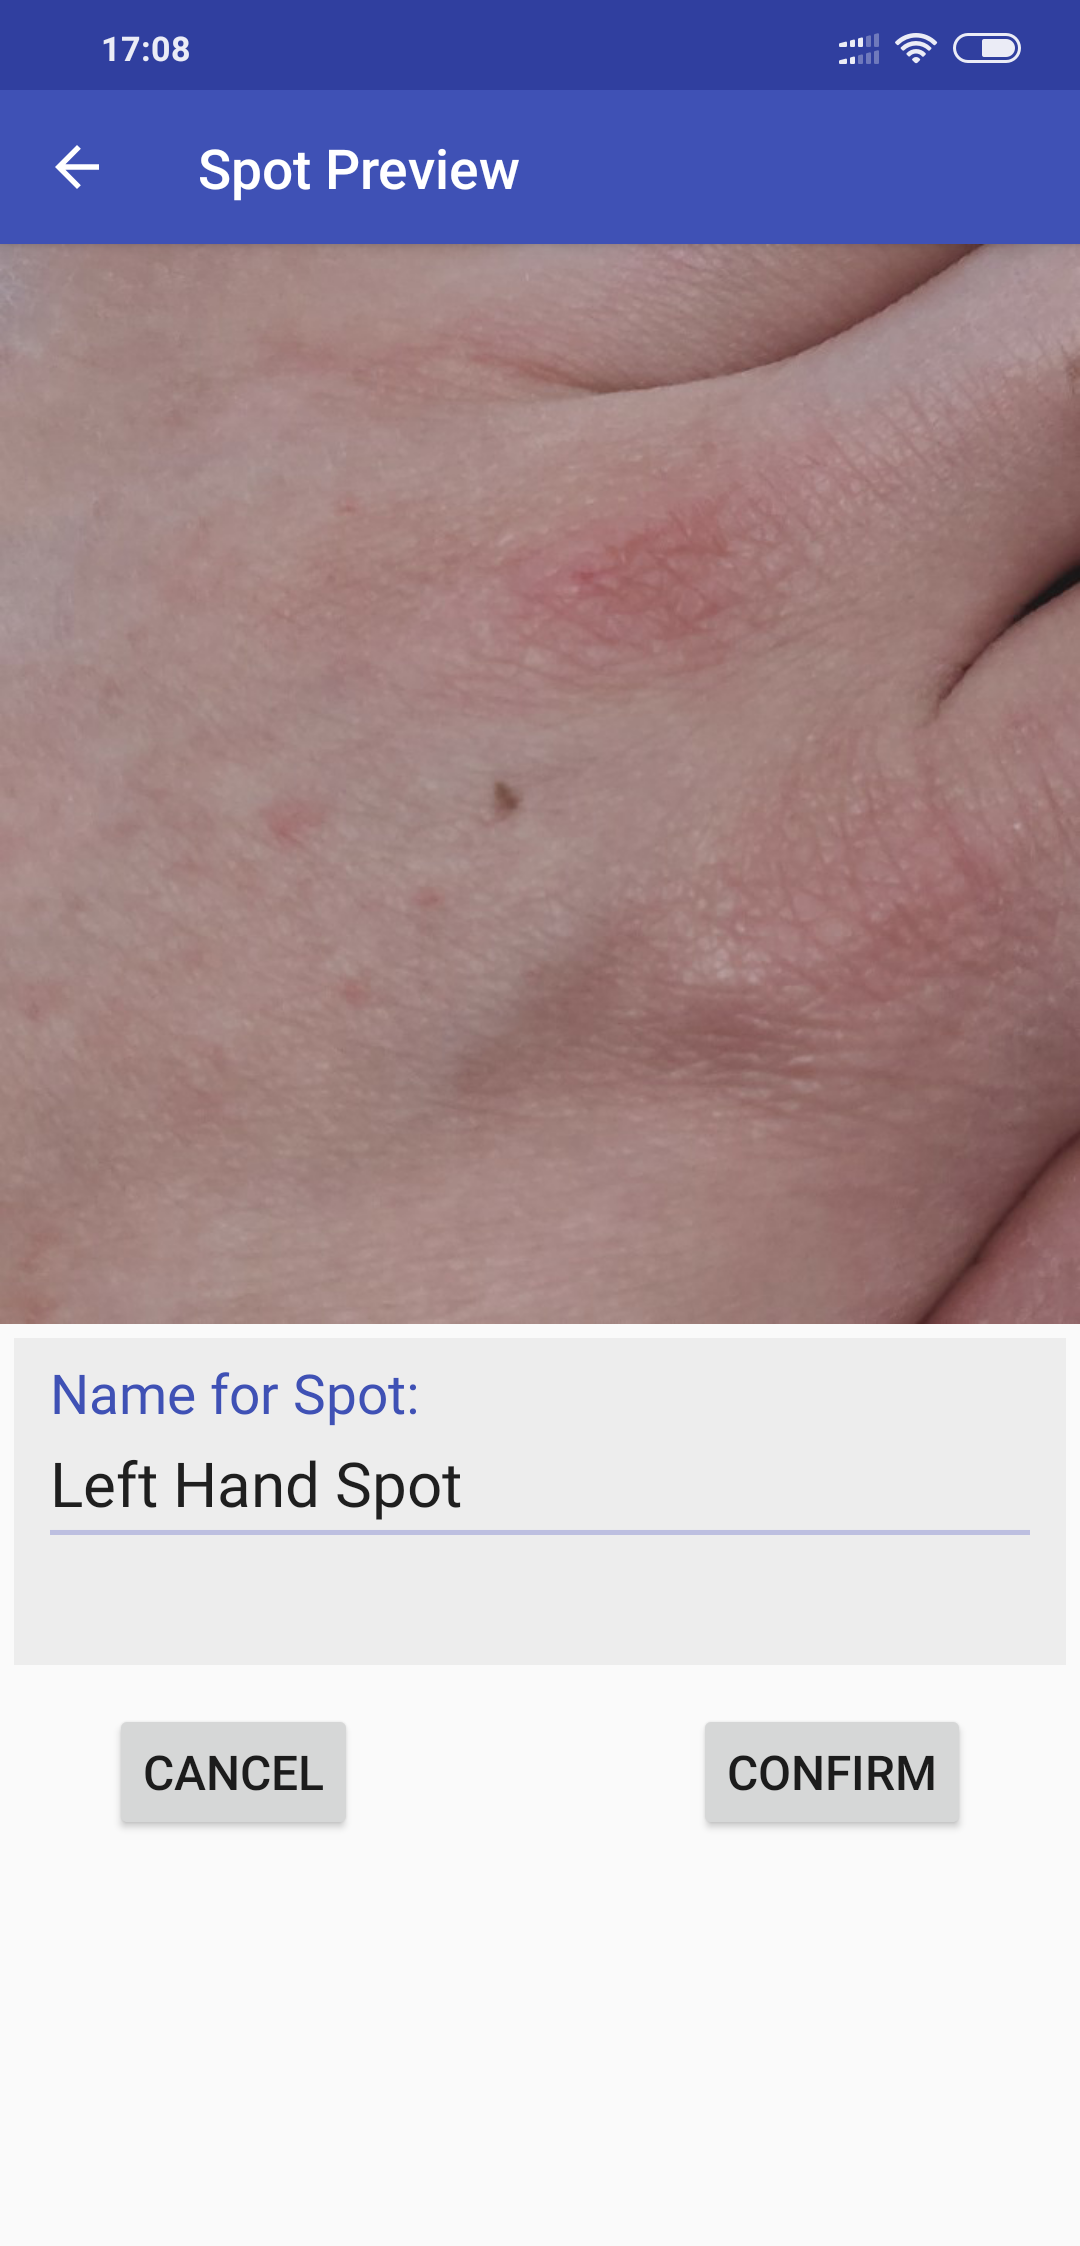
\includegraphics[height=10cm]{figures/confirmadd1.png}
        \caption{Redesigned AddSpot Activity Screen hiding the keyboard}
        \label{subfig:newaddspotkeyboard}
    \end{subfigure}%
     ~
    \begin{subfigure}[t]{0.5\textwidth}
        \centering
        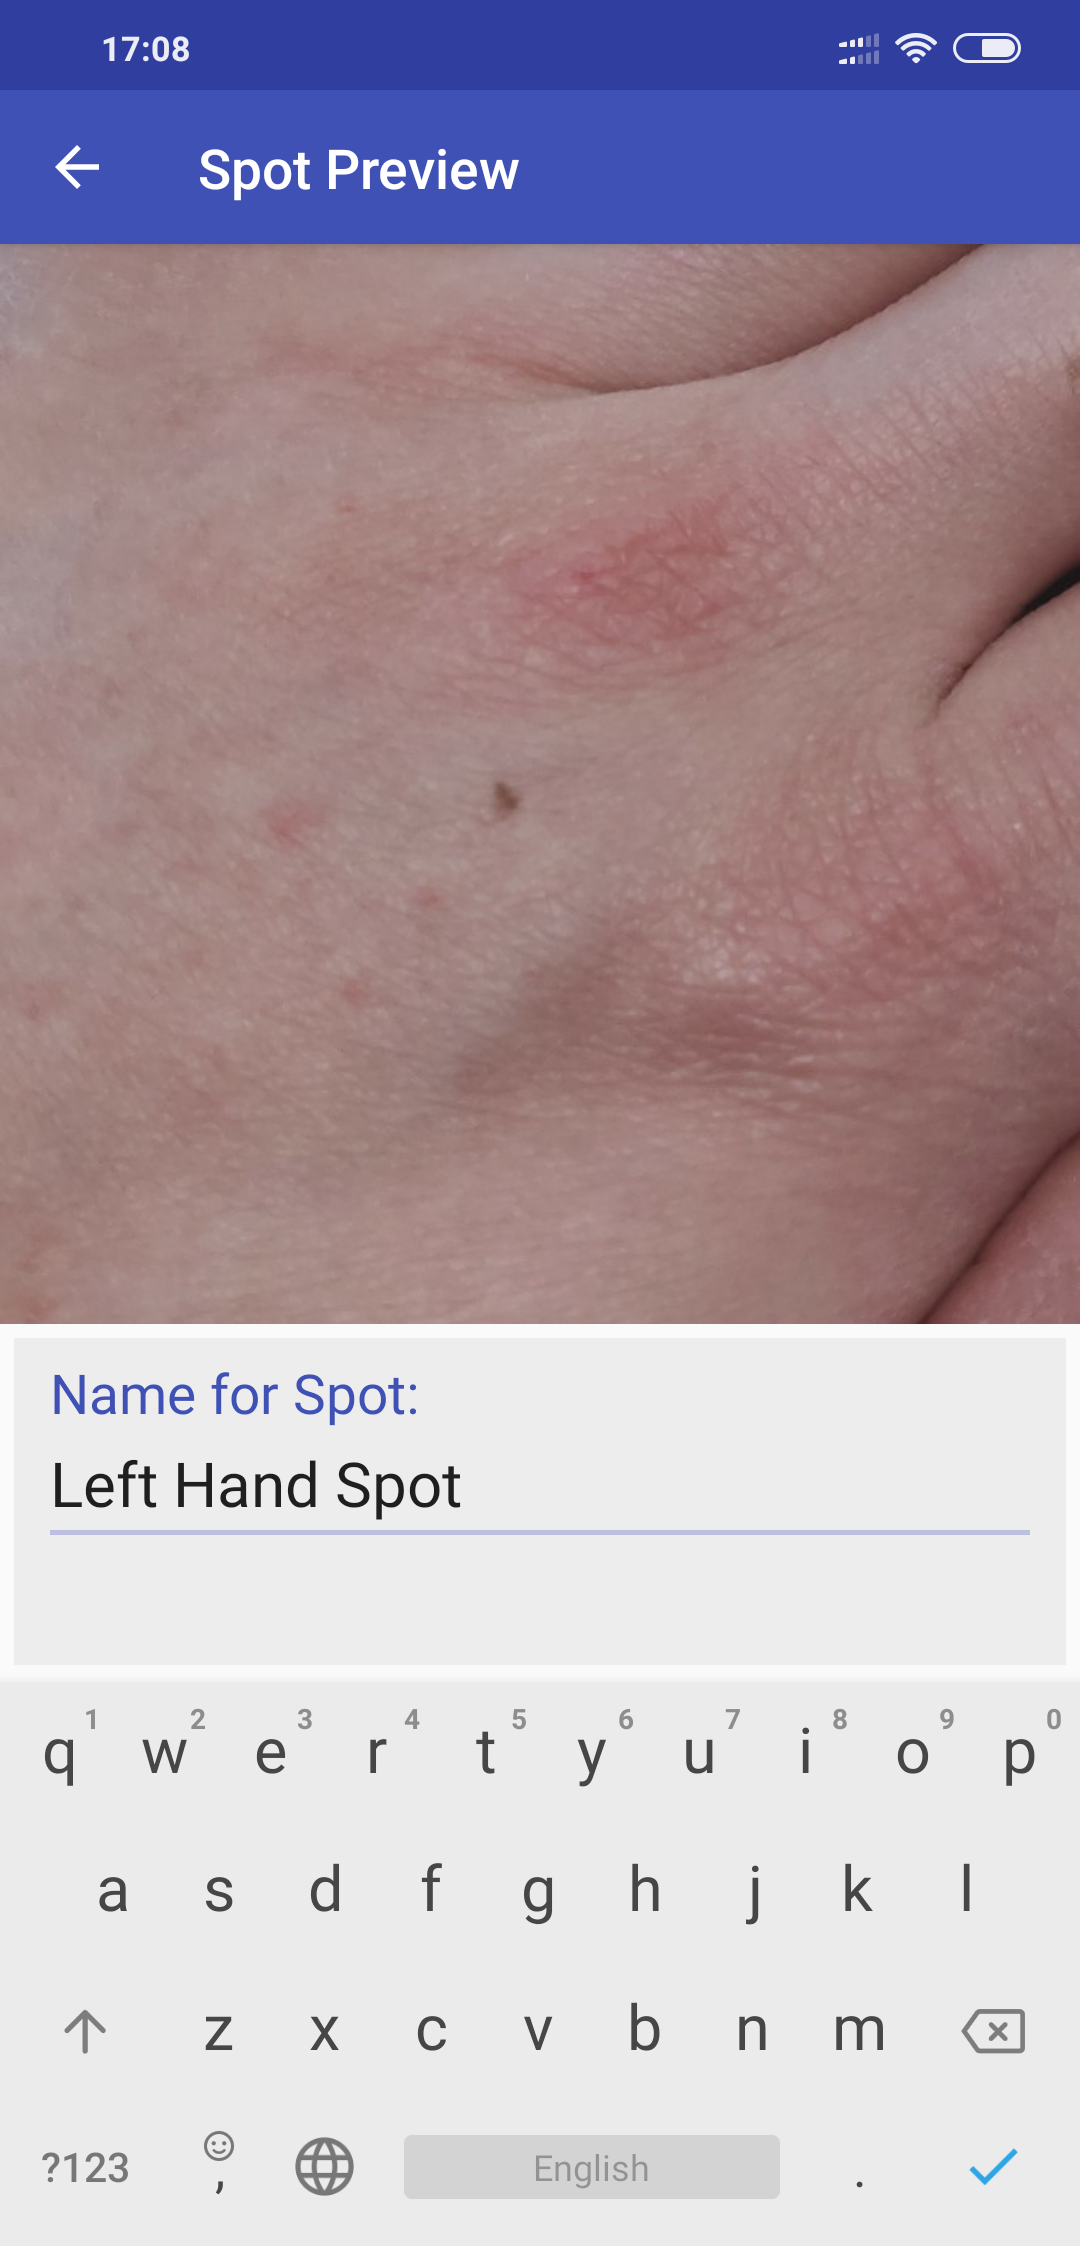
\includegraphics[height=10cm]{figures/addspot2.png}
        \caption{Redesigned AddSpot Activity after inputting text}
        \label{subfig:newaddspotnokeyboard}
    \end{subfigure}
    \caption{Progression of AddSpot Activity screens}
\end{figure*}

\subsection{Spot Image List Screen}

This screen displays a list of all taken photos of a spot (Figures \ref{subfig:spotimagelist} and \ref{subfig:spotimagelistcontext}), this enables the user to compare them over time, spotting any differences in appearance. Under the toolbar, a list of images is displayed. Each list item shows a thumbnail for each particular image, the name of the image, and the date on which the image was taken. The toolbar contains multiple action buttons, a back button to return to the previous screen, a "Compare" button to open the comparison contextual toolbar, and a "+" button to add a new photo to the list. Clicking on an item in the list would open a full-screen view of the image for better inspection.

When the user presses the first "Compare" button, the contextual action bar opens. This enters the user into selection mode, where tapping on any of the images highlight the image, indicating it has been selected. If two images are selected, the "Compare" button lightens up, taking the user to the side-by-side comparison screen.

When it comes to displaying the list of images, alternative design decisions for selecting spots to compare will be discussed in section \ref{CompareScreenDesignSection}. However, we can justify the choice of what information is displayed on each item. The thumbnail of each image is critical for the user to know which images they are selecting to compare, the name of each image contains the "JPEG" together with the timestamp of the photo. Arguably, this format could be more user friendly by including the name of the spot. This would require extra image renaming methods in the app implementation, but would further help the user identify images.

\begin{figure*}[t!]
    \centering
    \begin{subfigure}[t]{0.5\textwidth}
        \centering
        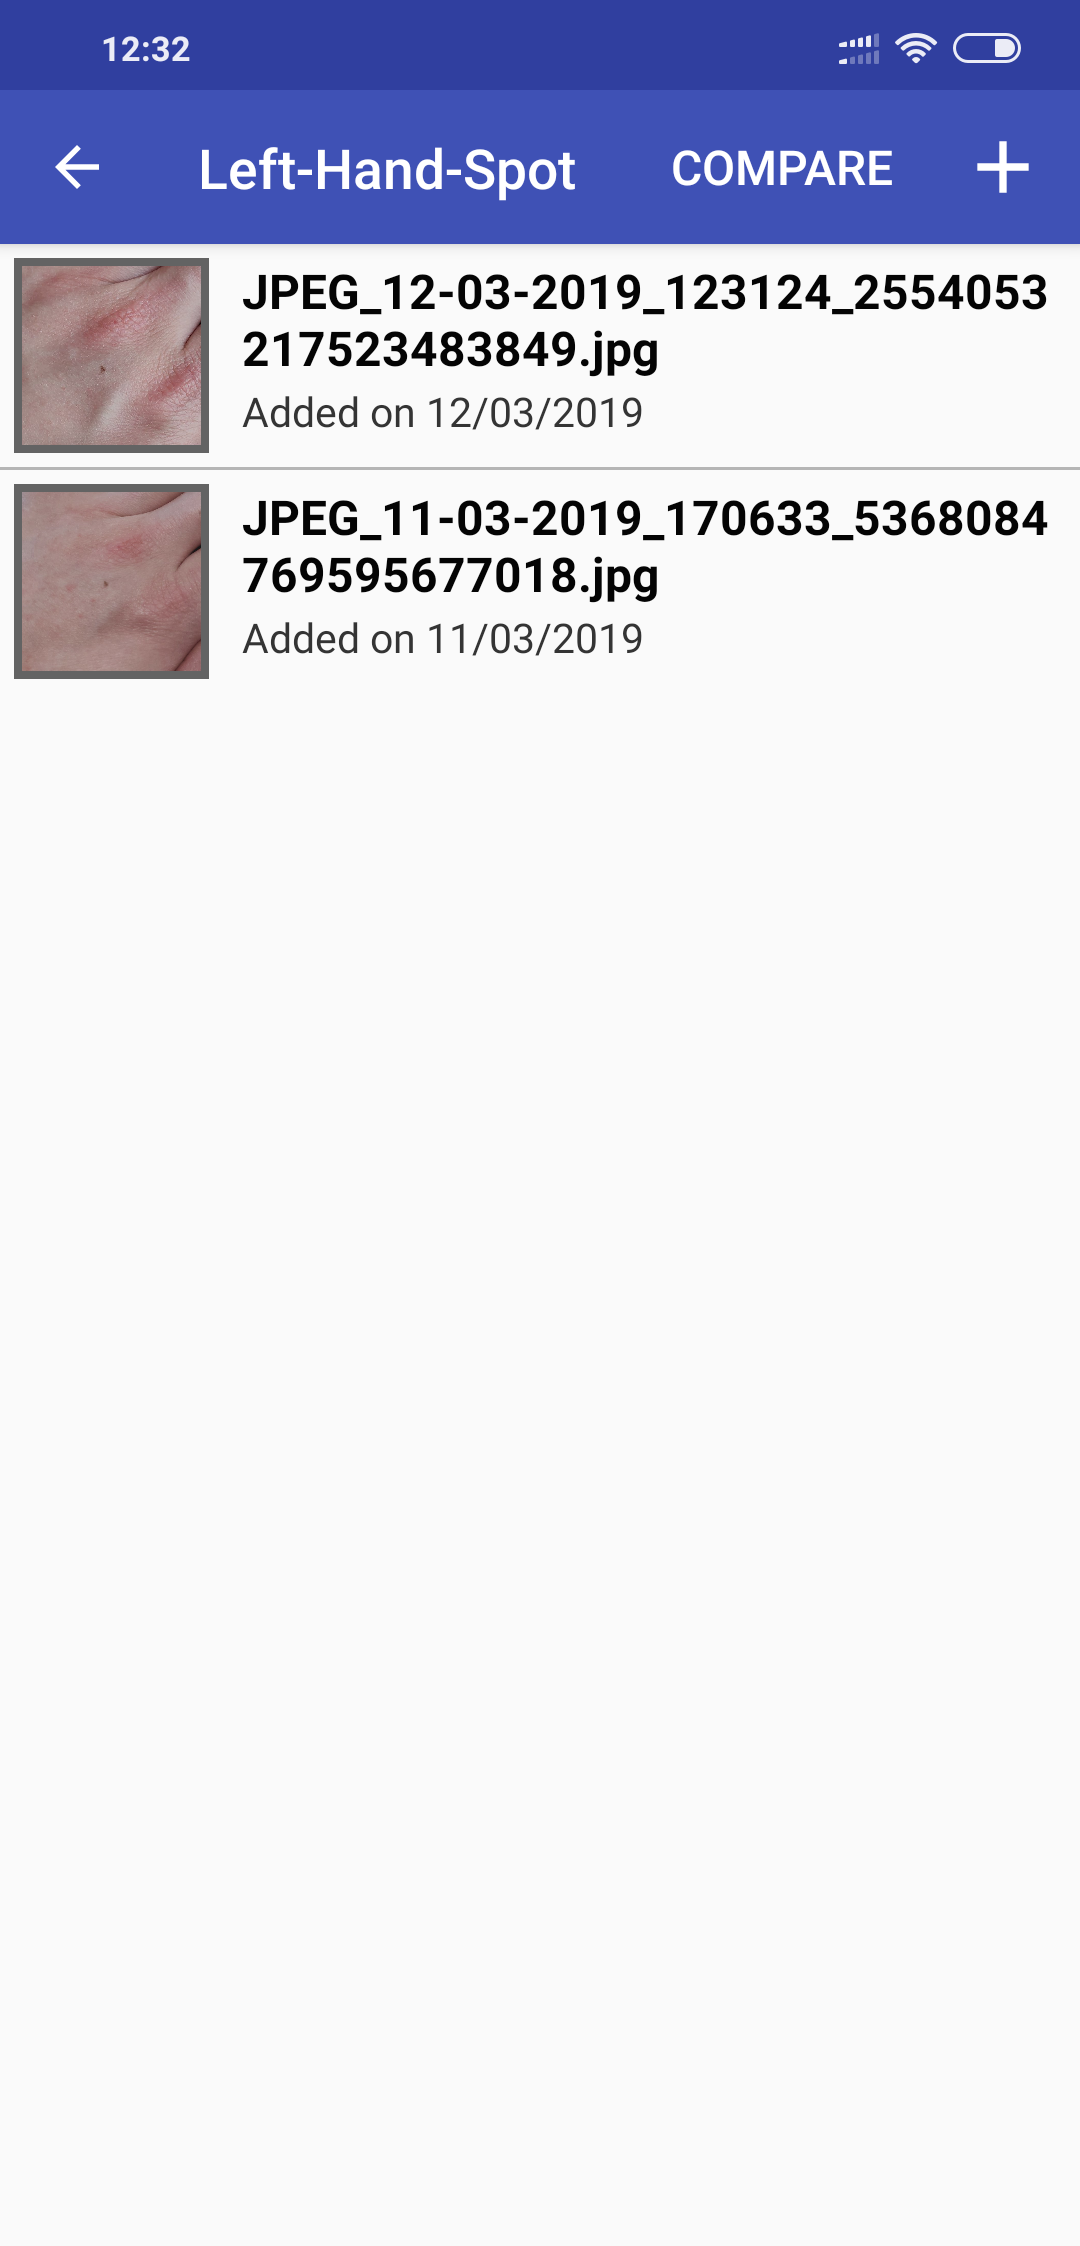
\includegraphics[height=10cm]{figures/spothistory2_android.png}
        \caption{List of images of a spot}
        \label{subfig:spotimagelist}
    \end{subfigure}%
    ~
    \begin{subfigure}[t]{0.5\textwidth}
        \centering
        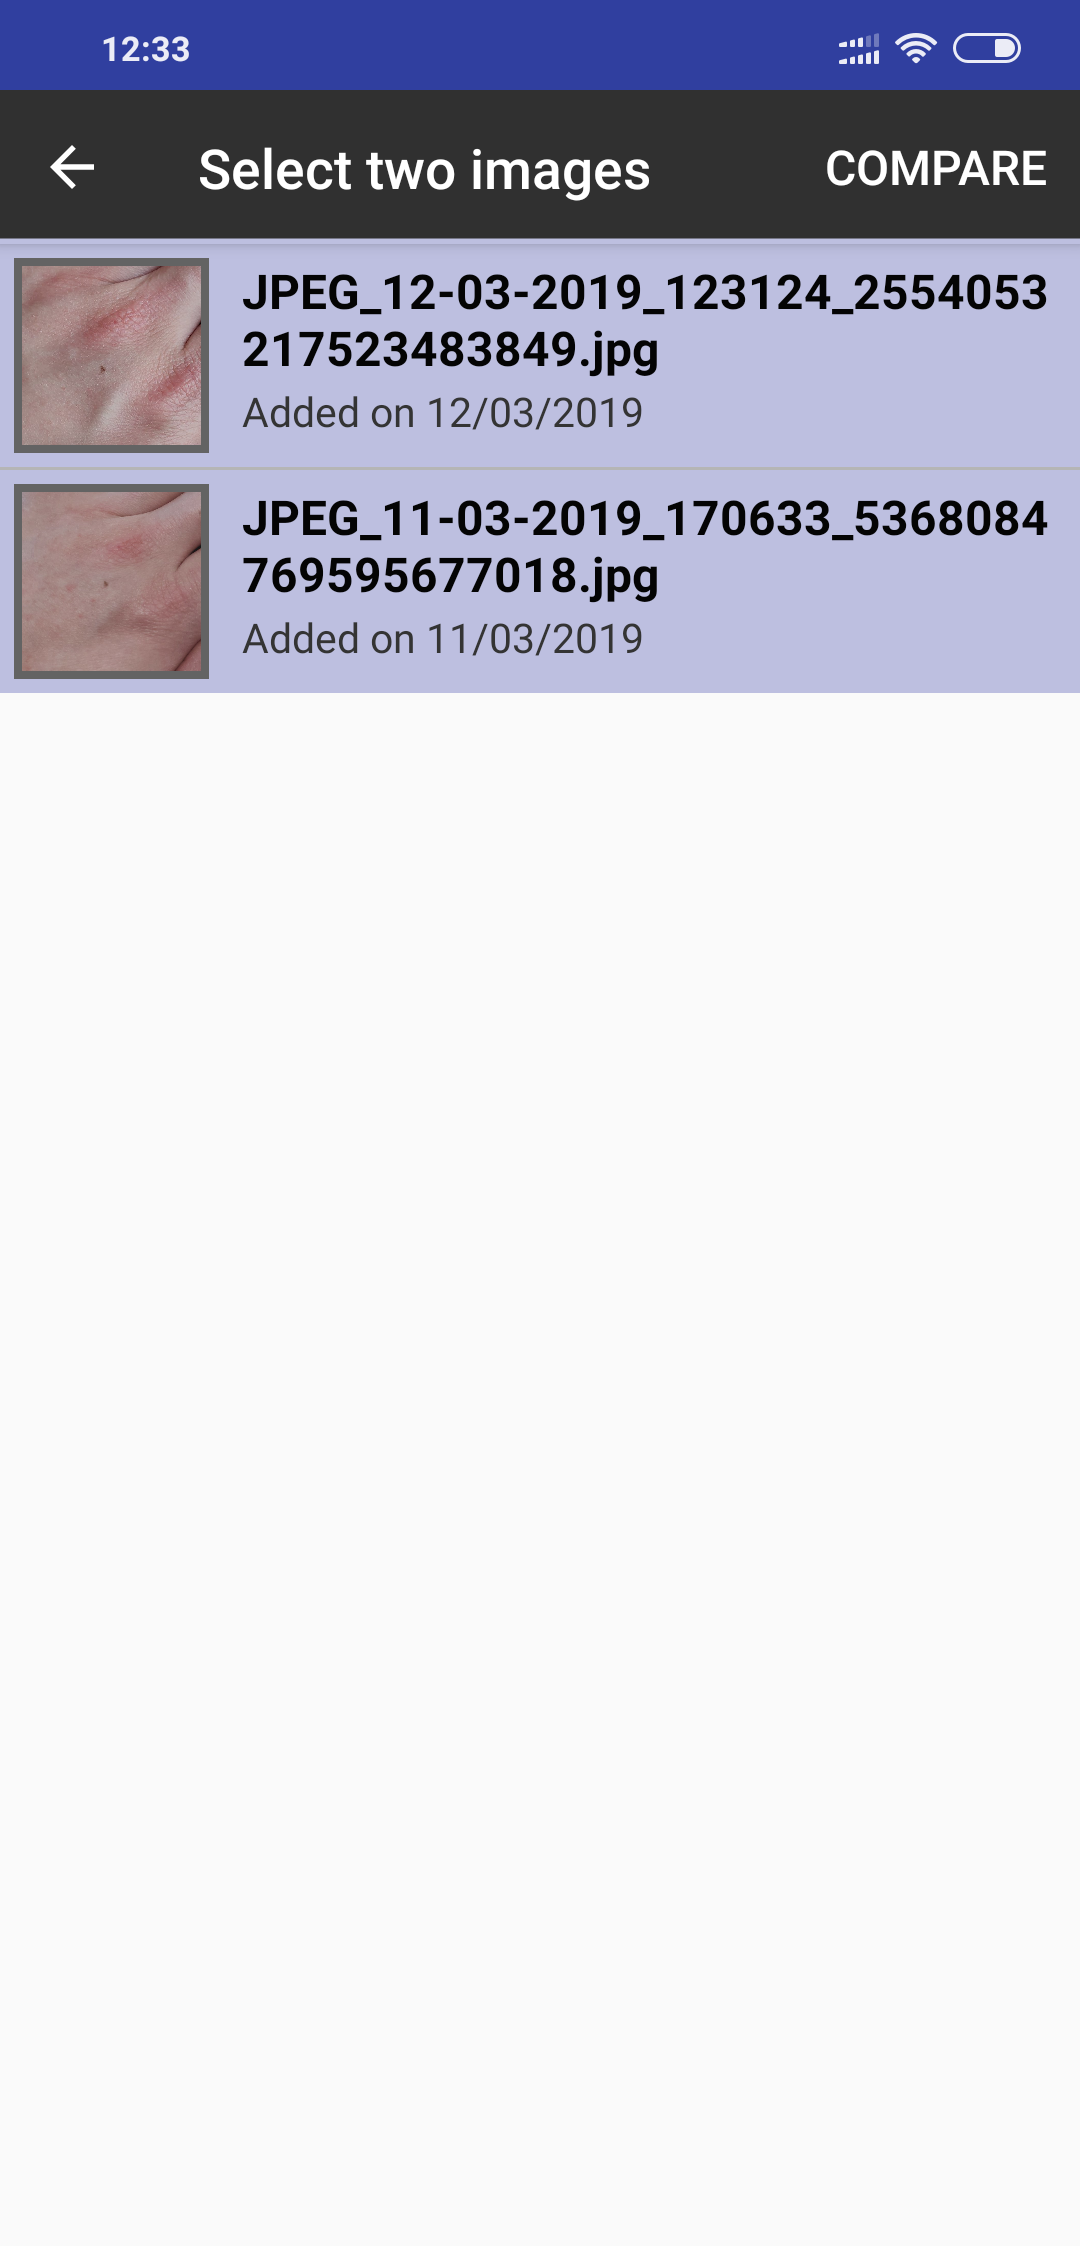
\includegraphics[height=10cm]{figures/compare1_android.png}
        \caption{Selecting images to compare}
        \label{subfig:spotimagelistcontext}
    \end{subfigure}
    \caption{SpotImageList Activity showing image selection for comparison}
\end{figure*}

\subsection{Comparing Spots Screen} \label{CompareScreenDesignSection}

The spot comparison screen (Figure \ref{fig:comparisonallfigures}) allows the user to closely inspect the differences between two previously selected images. It is the main feature that differentiates the app from a typical photo gallery app, also allowing the user to email both images to a doctor or user specified address.

A lot of thought was put into what the best way to compare images was. Two main approaches were considered. Figures \ref{fig:oldcompare1} and \ref{fig:oldcompare2} show the initial design, where all images are displayed in a "CarouselView", imitating a slideshow where the user can swipe left and right to compare all images. The main advantages and disadvantages of this design are highlighted below:
\begin{itemize}
    \item \emph{Smooth and Convenient} - Comparing images through swiping feels intuitive and natural to users.
    \item \emph{Memory Loss} - Continually loading all images of a spot can quickly exhaust the app's memory budget \cite{handlingbitmaps}. With certain older devices, issues still arise even after using efficient bitmap decoding libraries such as \emph{Glide}.
\end{itemize}

On the other hand, Figures \ref{subfig:spotimagelistcontext} and \ref{fig:newcompare1secondfig} show the second (and final) design for comparing images. This approach requires images to be selected in the spot image list screen and displays them statically one above the other. Each image takes up 50\% of the screen. Thoughts about this approach:
\begin{itemize}
    \item \textbf{Image Count} - It is unlikely for users to save more than 5 images of a spot. The appeareance of spots usually takes several months or years to change. This means that the user will not necessarily need to compare \textbf{all} the images of a spot, but the very first and last images would suffice.
    \item \textbf{Closer Zoom} - Loading only two images avoids any memory leaks, and removing the swipe interaction means images can take up the whole screen, enabling the user to inspect and compare the spots more easily.
    \item \textbf{Clunky Feel} - Selecting spots through a selection menu can feel more cumbersome to some users.
\end{itemize}

\clearpage
\begin{figure*}[t!]
    \centering
    \begin{subfigure}[t]{0.5\textwidth}
        \centering
        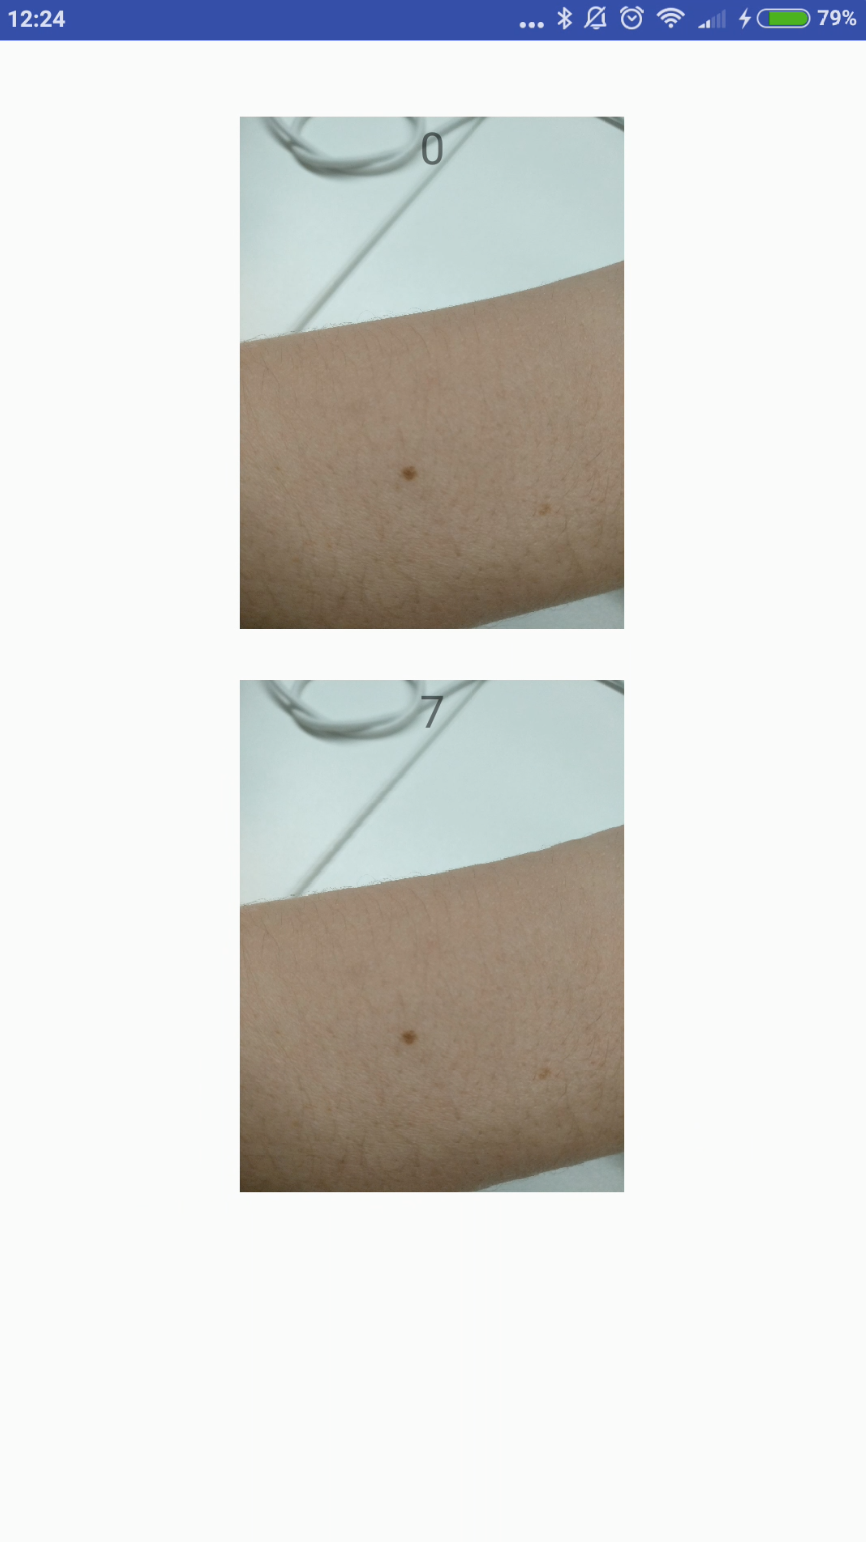
\includegraphics[height=10cm]{figures/oldcompare1.png}
        \caption{Display of initial compare screen design}
        \label{fig:oldcompare1}
    \end{subfigure}%
    ~
    \begin{subfigure}[t]{0.5\textwidth}
        \centering
        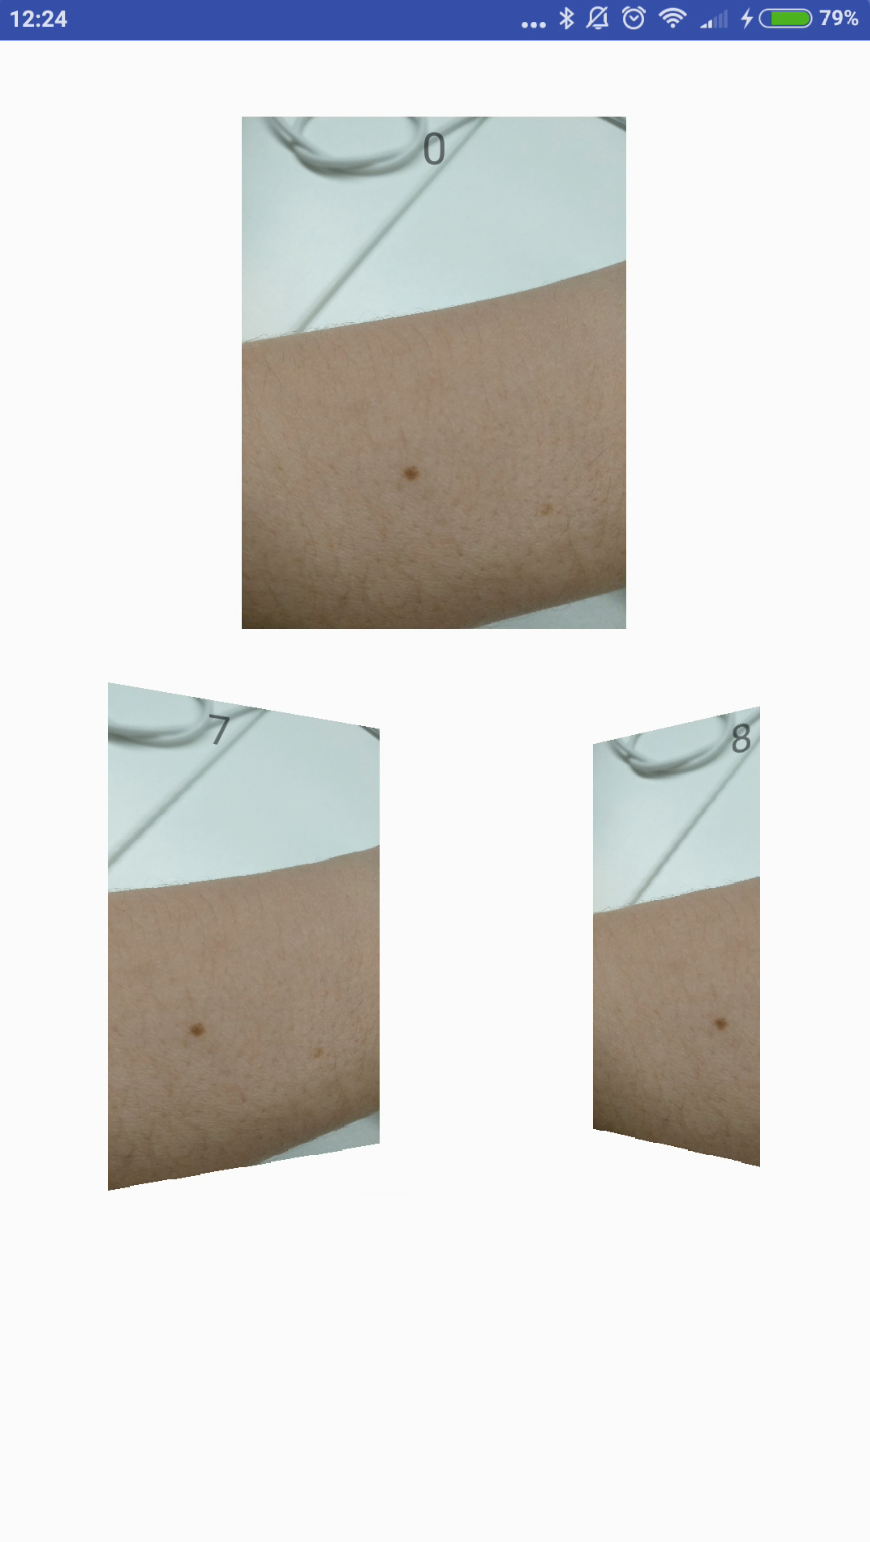
\includegraphics[height=10cm]{figures/oldcompare2.png}
        \caption{Comparing images can be done through swiping left and right}
        \label{fig:oldcompare2}
    \end{subfigure}
    \begin{subfigure}[t]{0.5\textwidth}
        \centering
        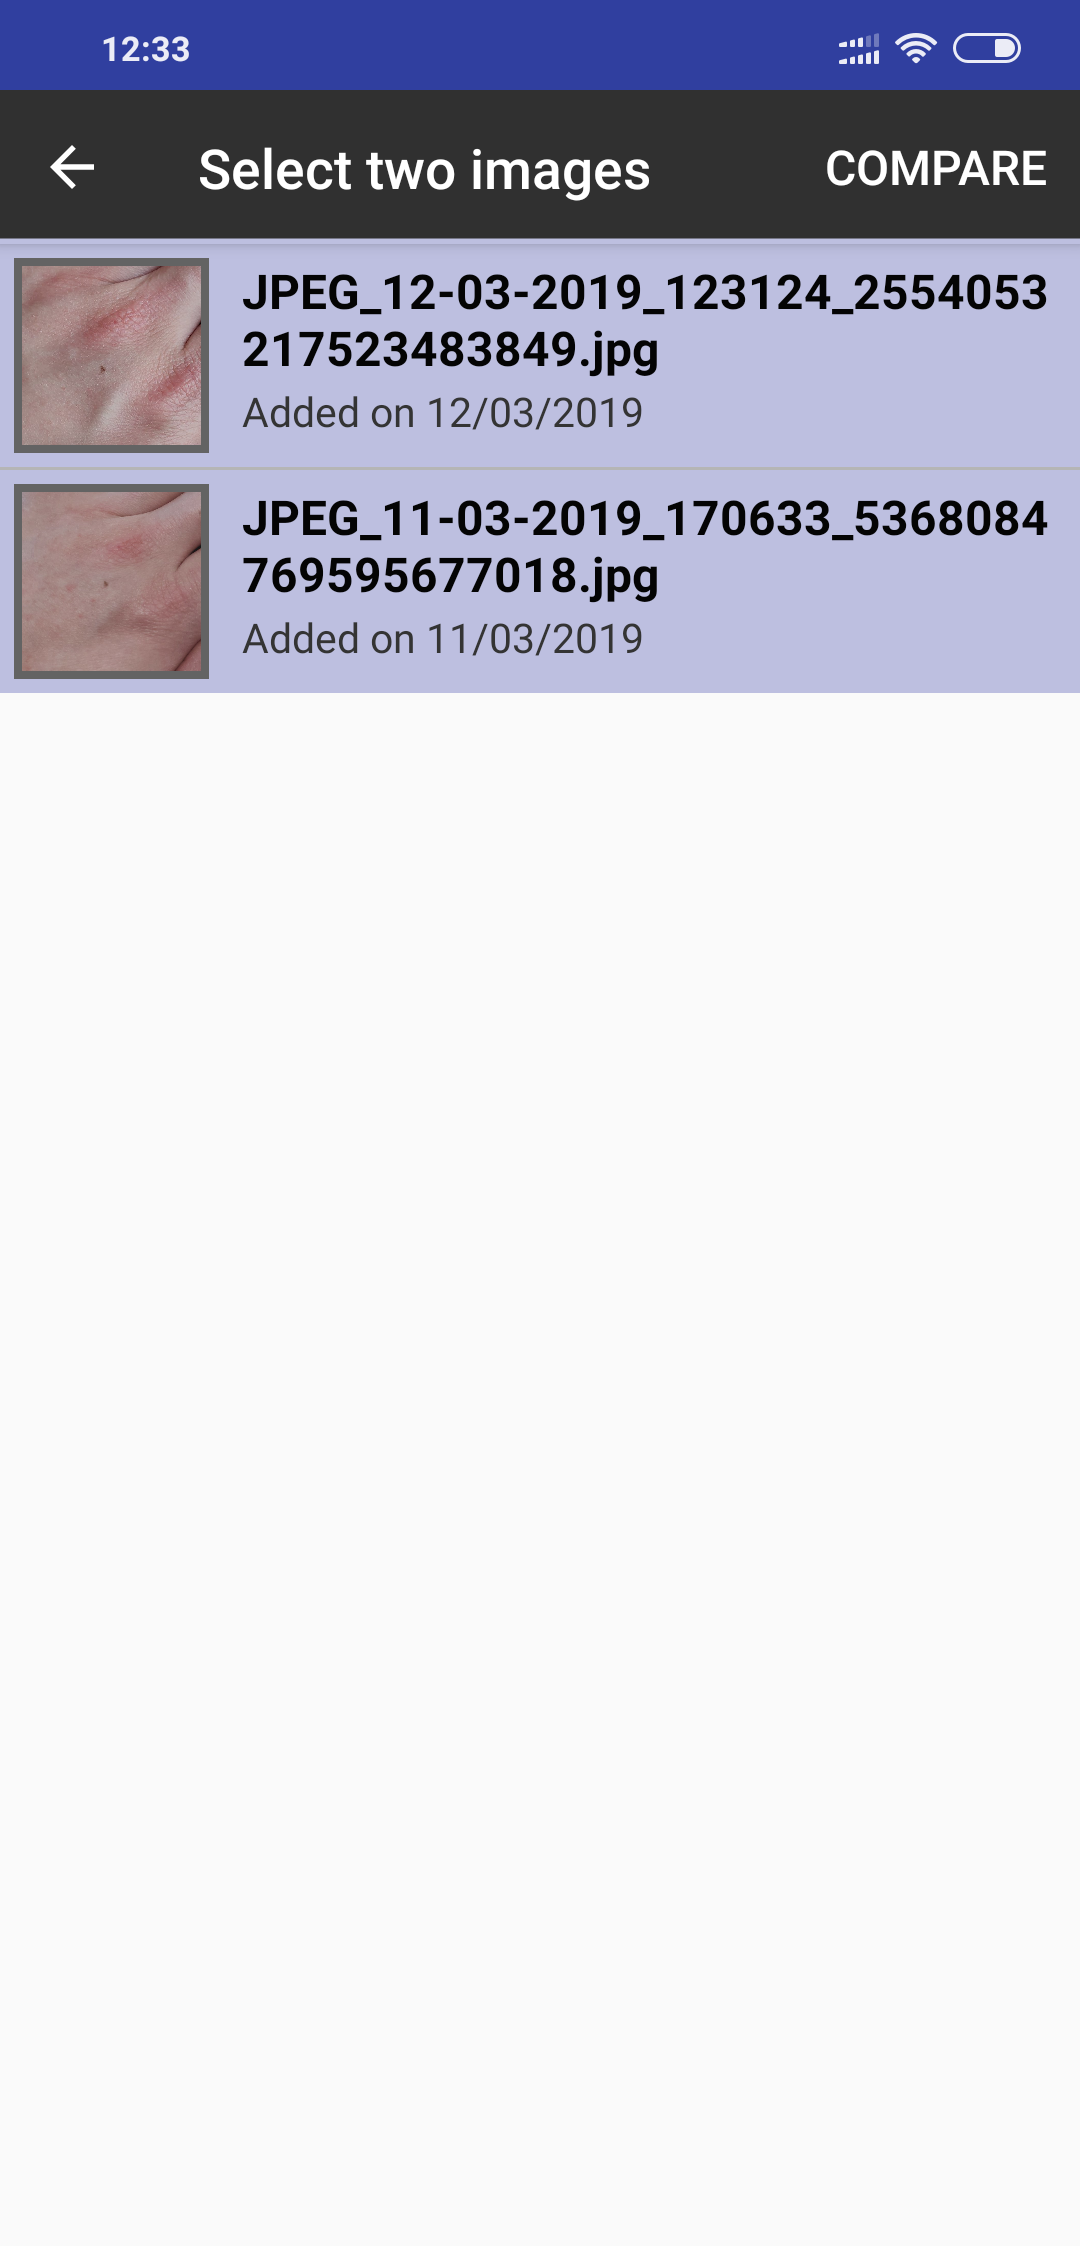
\includegraphics[height=10cm]{figures/compare1_android.png}
        \caption{Final compare screen image selection}
        \label{fig:newcompare1secondfig}
    \end{subfigure}%
    ~
    \begin{subfigure}[t]{0.5\textwidth}
        \centering
        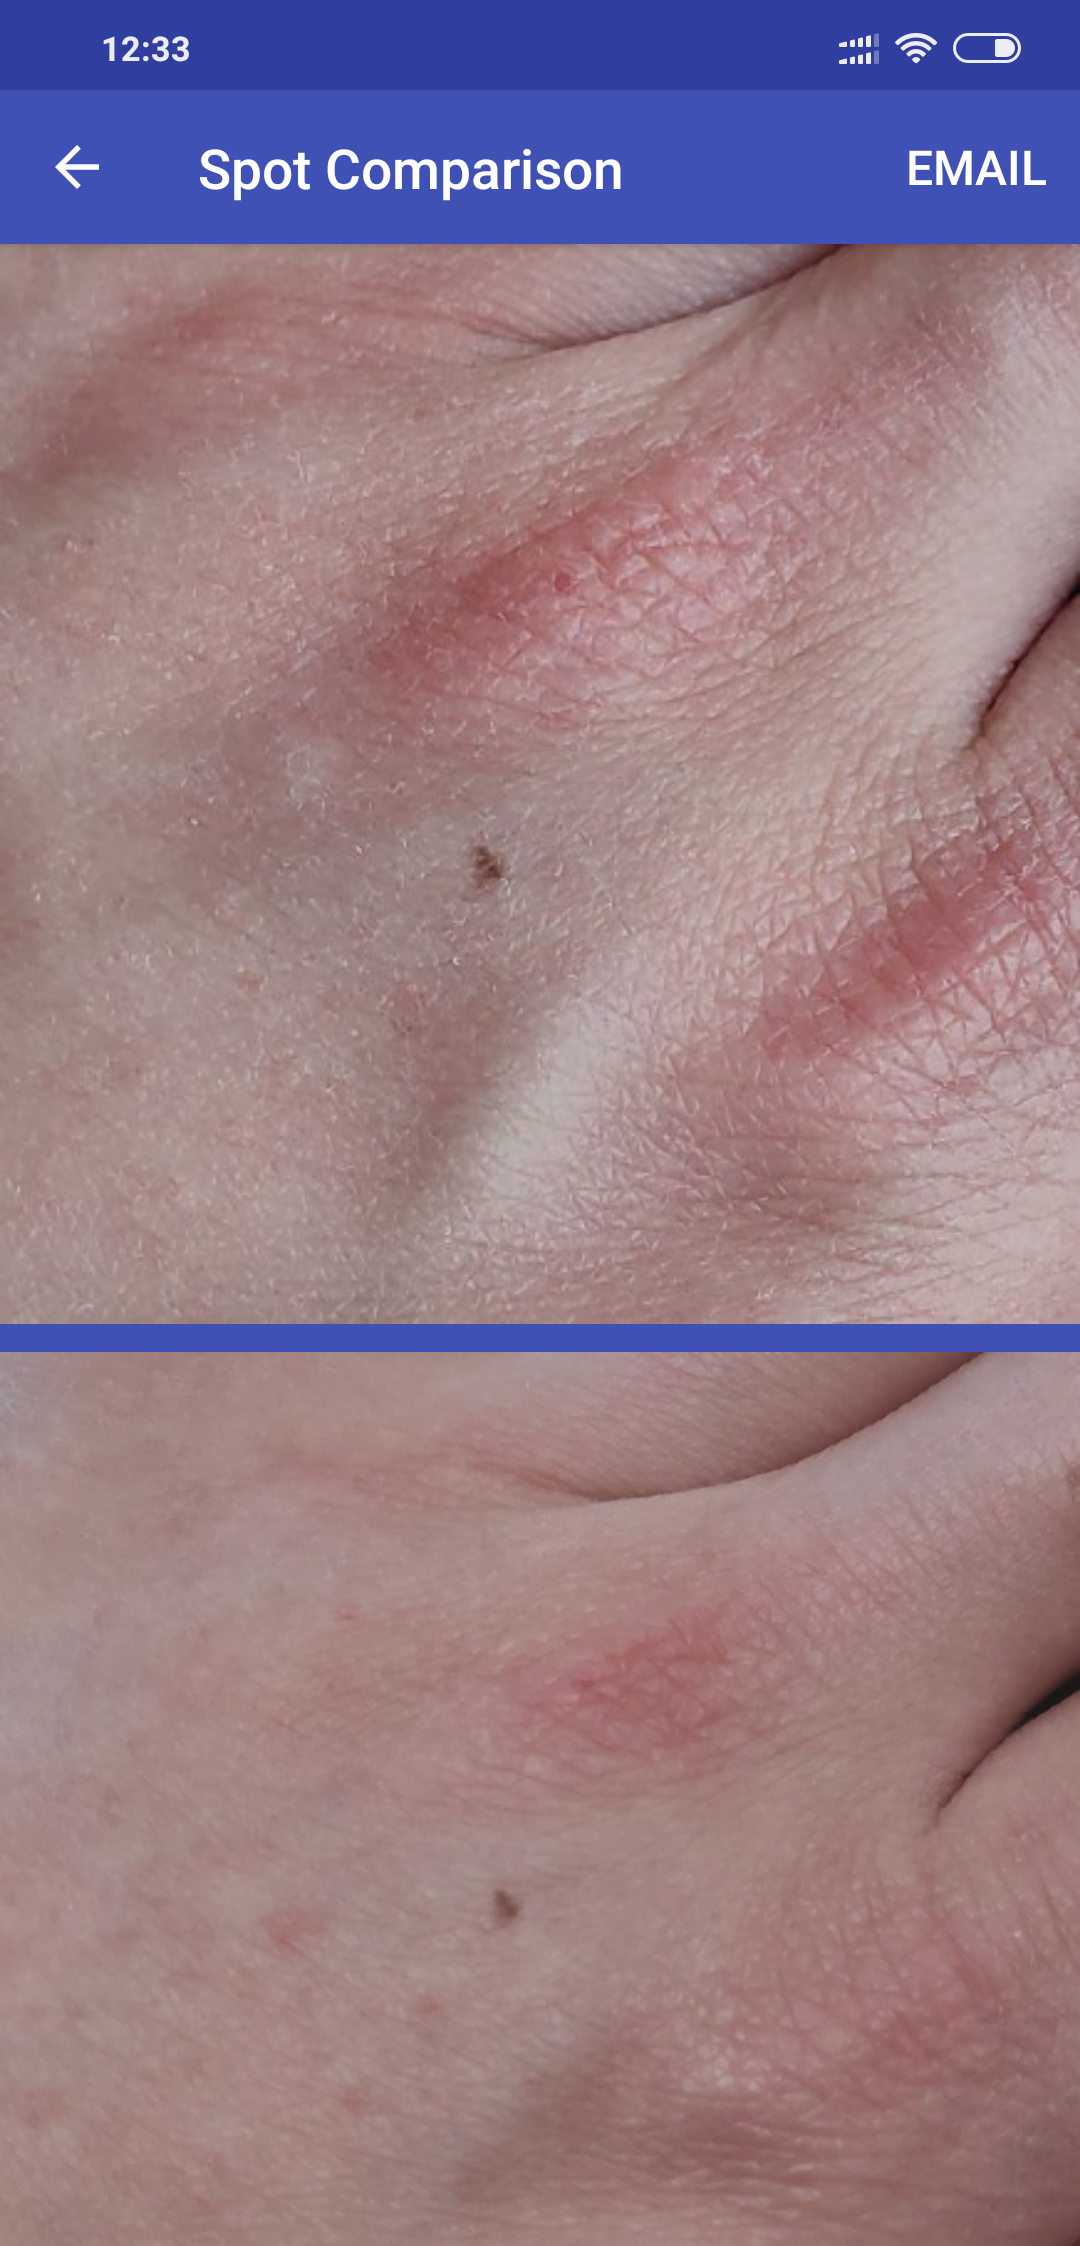
\includegraphics[height=10cm]{figures/compare2_android.png}
        \caption{Final design for comparing spot images}
        \label{fig:newcompare2}
    \end{subfigure}
    \caption{Progression of the Spot Comparison Screen}
    \label{fig:comparisonallfigures}
\end{figure*}

\subsection{Email Screen}
This screen is used to email the compared images to a doctor or another specified email address. There is no control over the design of this screen, as the "Email" button on the comparison screen simply opens a new email on the default email app on the user's device. The app automatically attaches both selected images and inserts a template text body (Figure \ref{fig:emailscreen}). 

\begin{figure}
    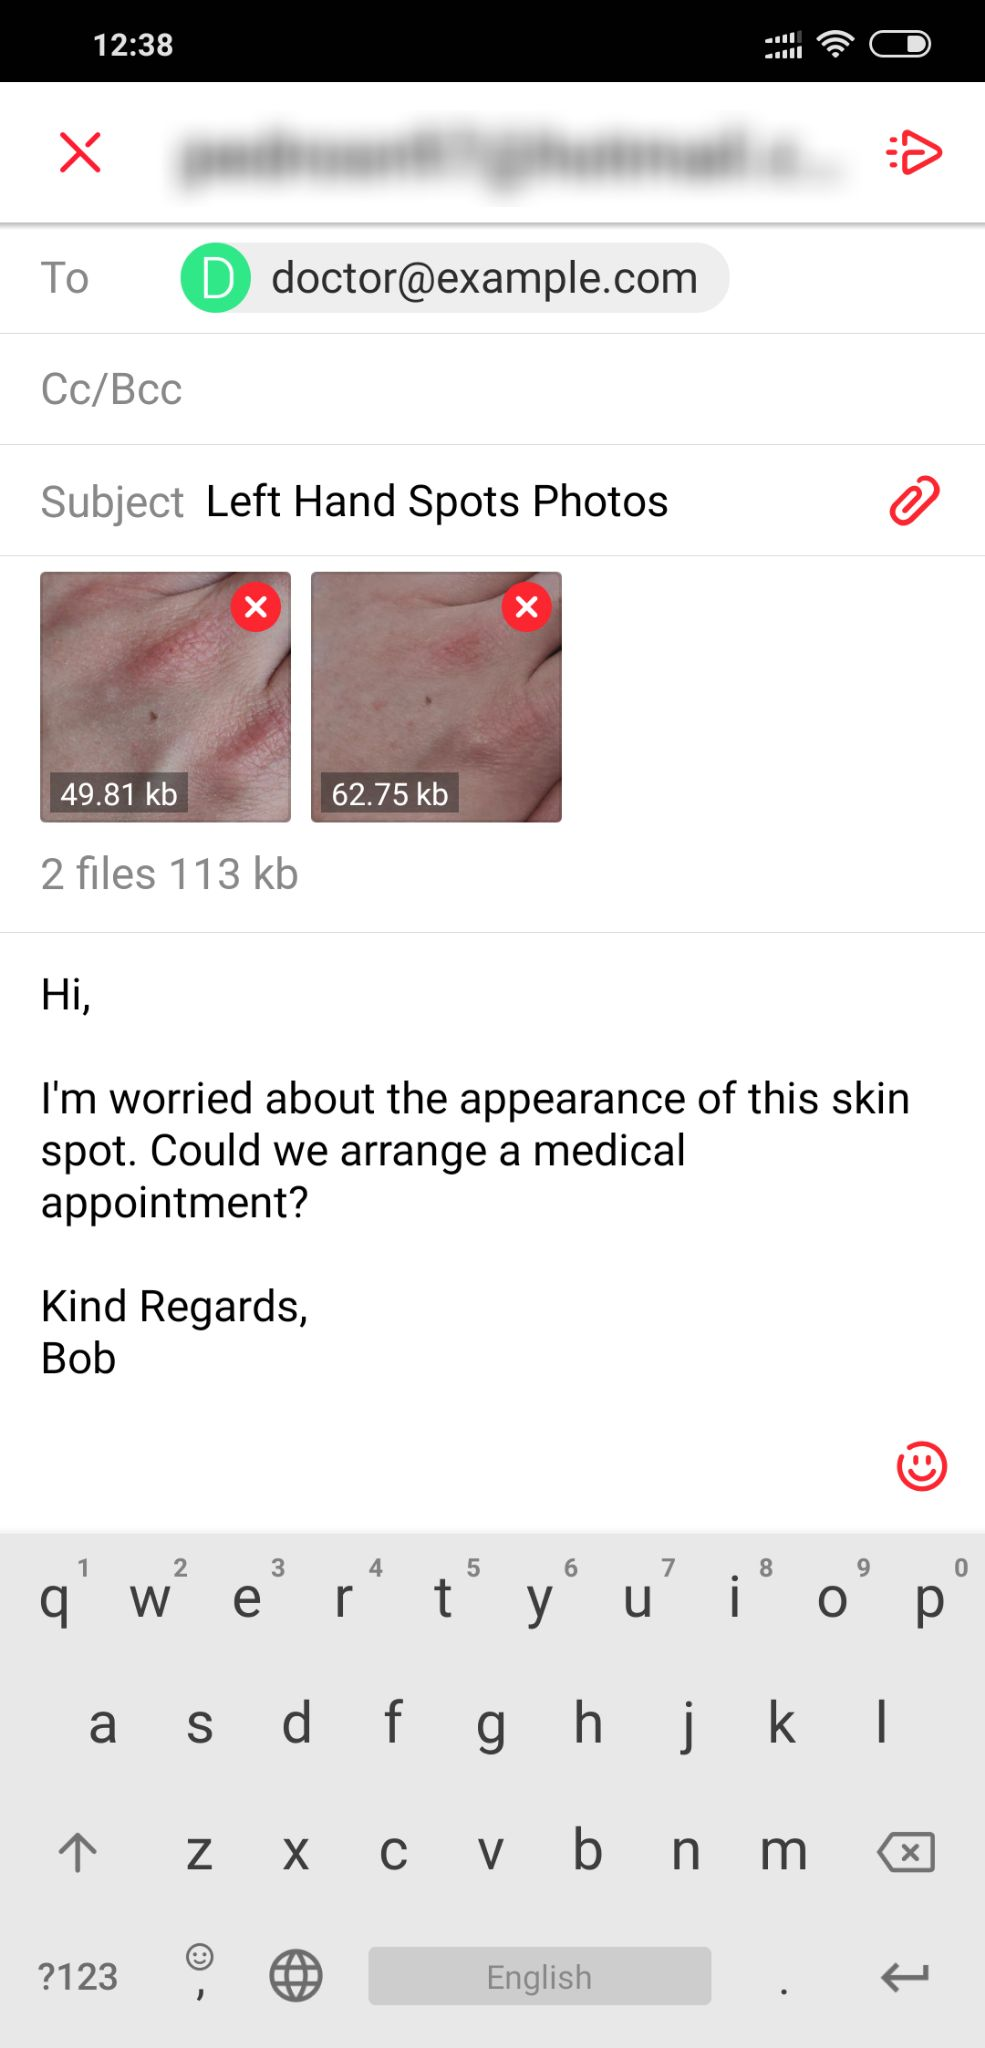
\includegraphics[height=10cm, center]{figures/email_android.jpg}
    \caption{Email Screen through the \emph{myMail} Android App}
    \label{fig:emailscreen}
\end{figure}

\section{Interactions}
\subsection{Navigation}
The app's navigation overview can be observed in Figure \ref{fig:nav_graph}, to summarise the interaction between the previously described screens: the app's home screen is the front perspective of the body screen. However, if the app has never been used before, the Information Screens will be displayed, giving the user a simple introduction to the app with some background information. From the home screen, the user can click on a body part to open the Old Spot screen for that body part, this would display a list of spots. The user can either add a new spot (Starting the Camera-Crop Process) or view a spot by tapping it. Tapping takes the user to the spot image list for the selected spot, following a similar design to the old spot screen, but in this case showing all the images for a particular spot. The user can select two images to compare (as shown in the Compare Screen), or once again start the Camera-Cropping process to add a new image of the spot. In the Compare Screen, the user can also choose to email both images to a specified email address.

As a recall from the technical requirements of the project, the goal was to develop an app with the following features:
\begin{enumerate}
        \item The user can add and name new spots. Subsequently, the user can add new images to a spot.
        \item The user is able to compare two images of a spot on the same screen.
        \item The ability to email both pictures to a doctor from within the app.
        \item Educational information screens towards skin cancer signs and usage of the app.
    \end{enumerate}
From a design perspective, all the core features have been accounted for, relying the success of the project on how successful we are at implementation and evaluation of the app.

\subsection{Navigation Redesign}
\label{nav_refactor}

The app's home screen and overall navigation was altered midway through the project. Initially, the app would welcome the user through a typical home screen menu. Figure \ref{fig:draft1menu} shows the layout of this home screen. The first 3 buttons would all lead to the body screen, after which either the camera or list of spots would be displayed (depending on the main menu option selected). As would seem apparent, this design is very redundant, as all three options would essentially lead the user to the same screens. This lead to re-factoring the whole design of the app, shifting towards a body interface home-screen (Figure \ref{fig:nav_graph}). From this point, actions to add spots, add photos, or compare spots had to be implemented within the \emph{OldSpotScreen} and \emph{SpotImageScreen} Activities, since the user woudn't be selecting these from the main menu. Benefits and drawbacks of this approach include:
\begin{itemize}
    \item \textbf{Decrease redundancy} - The user doesn't have to go through the same 2 screens for every different action, saving time and delivering a more efficient interface 
    \item \textbf{Loss of clarity} - Having a main menu with options has its merits, as the user knows exactly what action they are currently doing, preventing them from getting lost within the app. This is particularly true with older users.
    \item \textbf{Flexibility} - The user can easily switch between actions without returning to the main menu, for example, if a user wanted to add a new spot A, then  add an updated photo of a different spot B, and finally compare two images of spot B, they could easily do this by entering the different body part spot lists, without requiring the user to return to the main menu screen three times.
\end{itemize}
Overall, the conclusion was that the main menu design in figure \ref{fig:firstappdraft} would only be suitable if users only completed 1-2 within every app use. With this unrealistic expectation, it was decided to shift to the body home screen design.
\clearpage
\begin{figure*}[t!]
    \centering
    \begin{subfigure}[t]{0.5\textwidth}
        \centering
        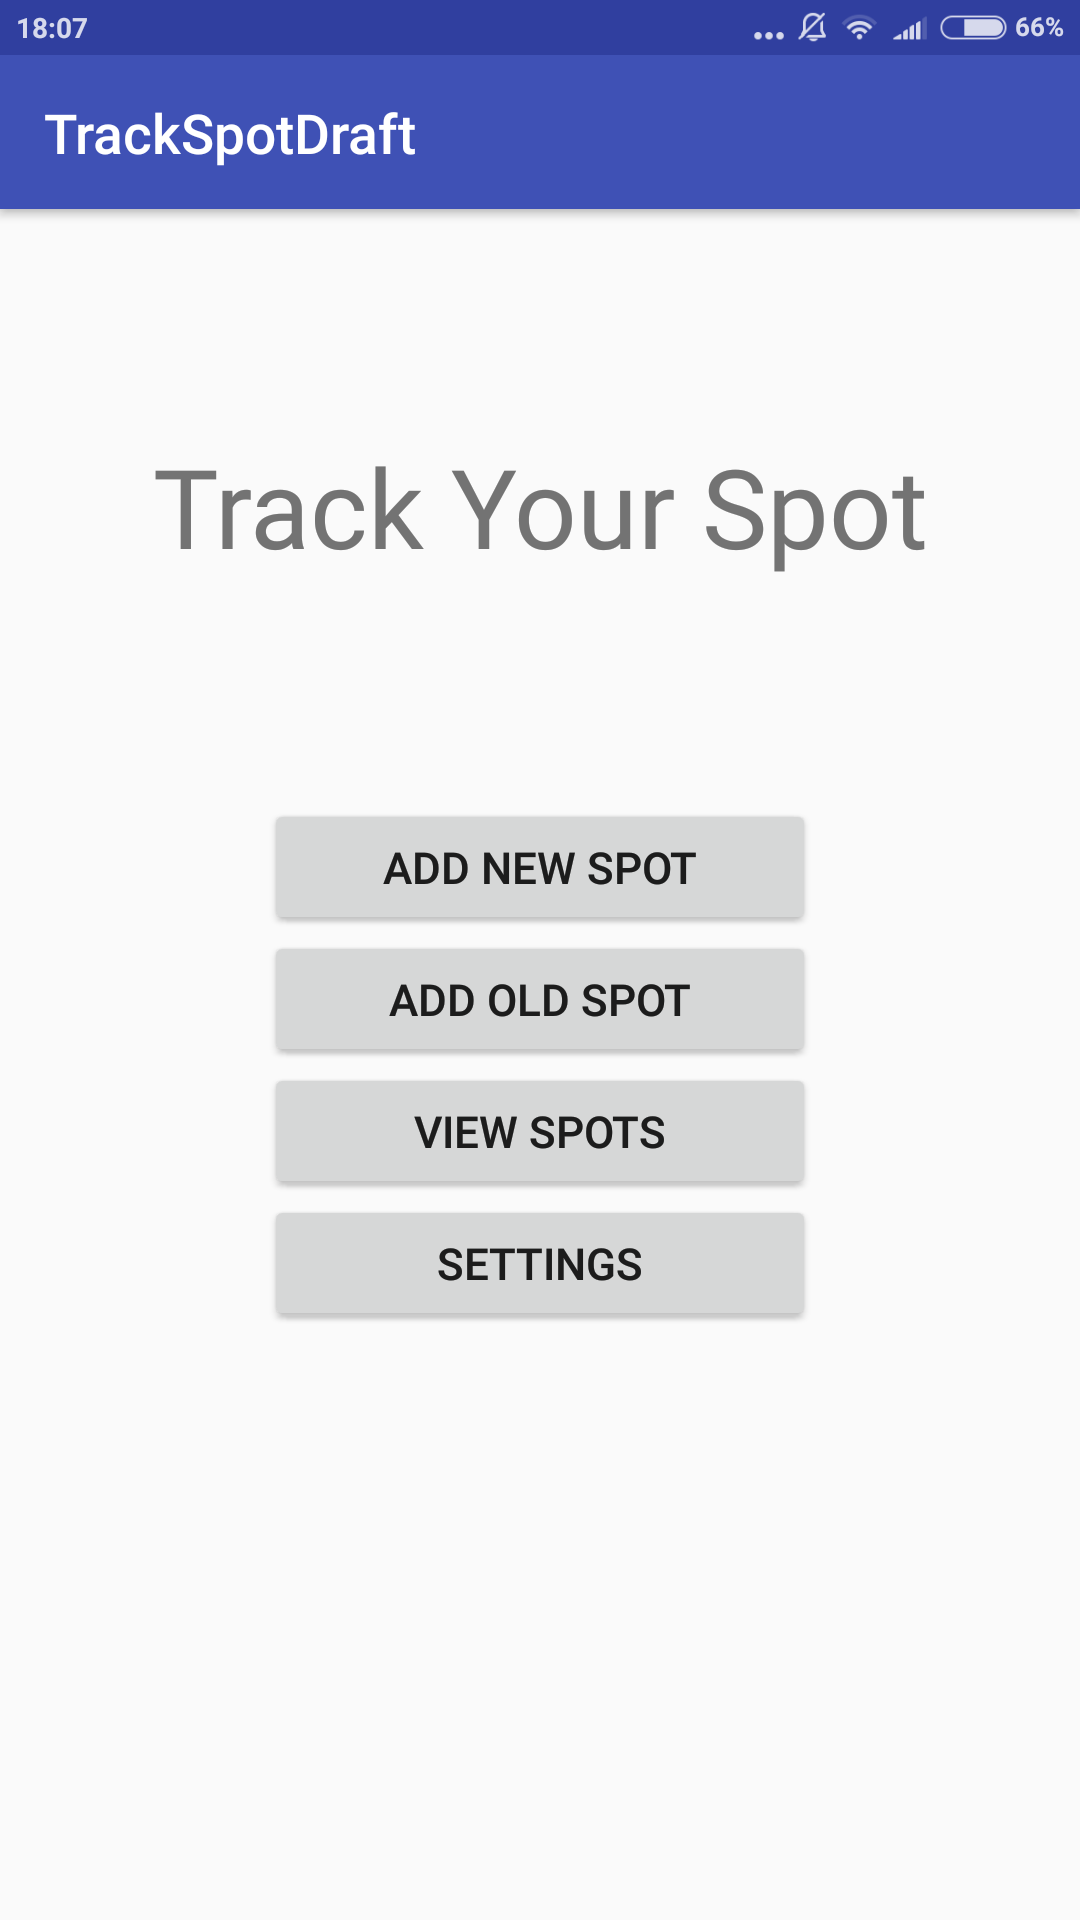
\includegraphics[height=10cm]{figures/draft1menuscreen.png}
        \caption{First app draft home screen}
        \label{fig:draft1menu}
    \end{subfigure}%
    ~
    \begin{subfigure}[t]{0.5\textwidth}
        \centering
        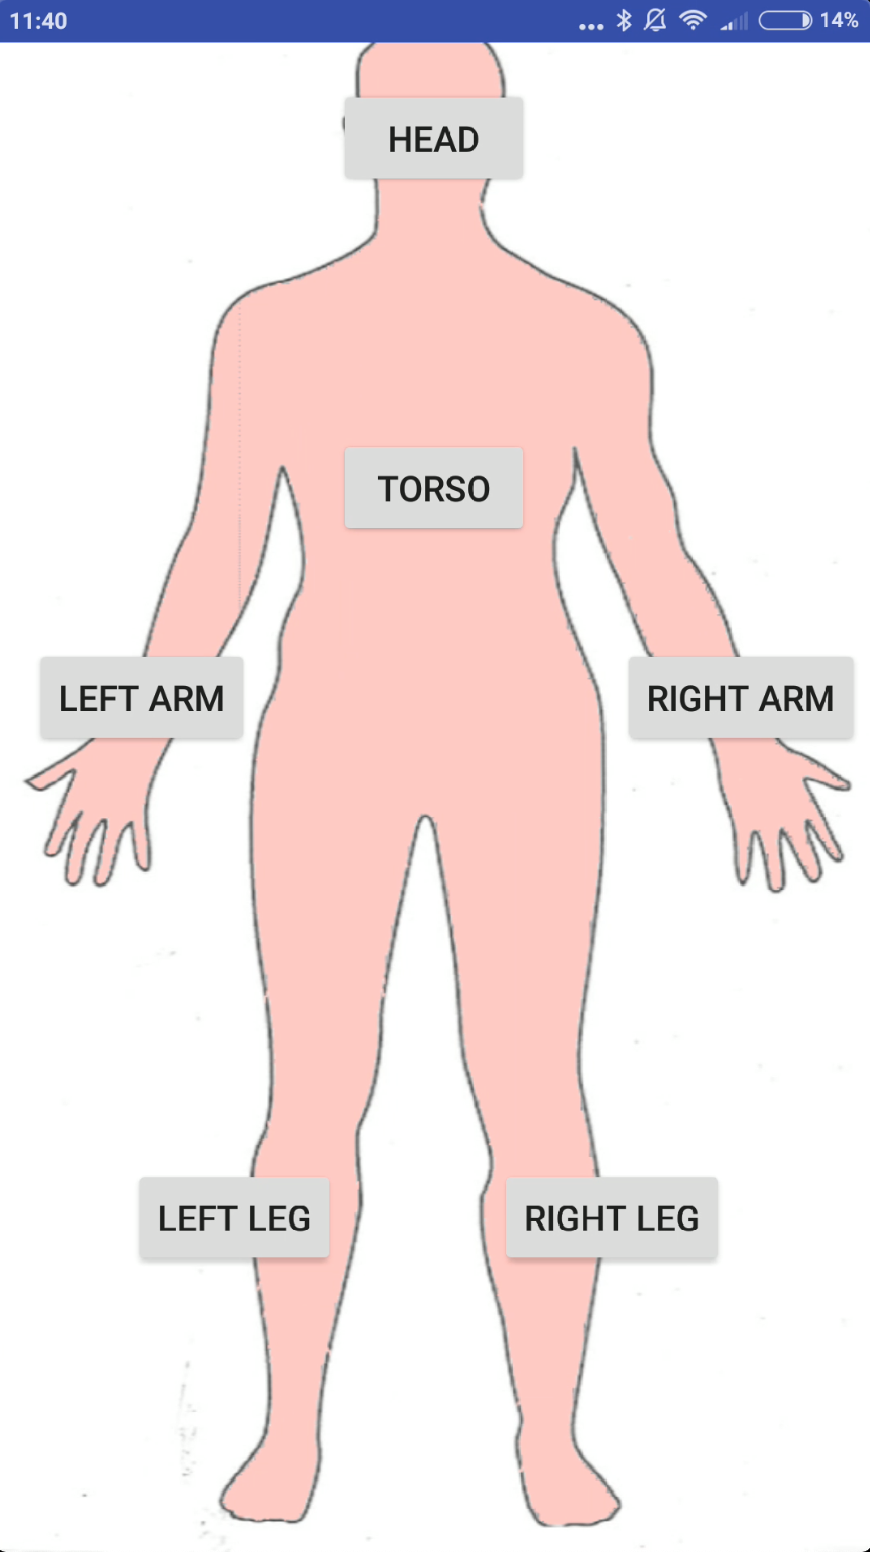
\includegraphics[height=10cm]{figures/draft1bodyscreen.png}
        \caption{First app draft body screen}
    \end{subfigure}
    \caption{Navigation menu of first app draft}
    \label{fig:firstappdraft}
\end{figure*}
\clearpage
\begin{figure}
    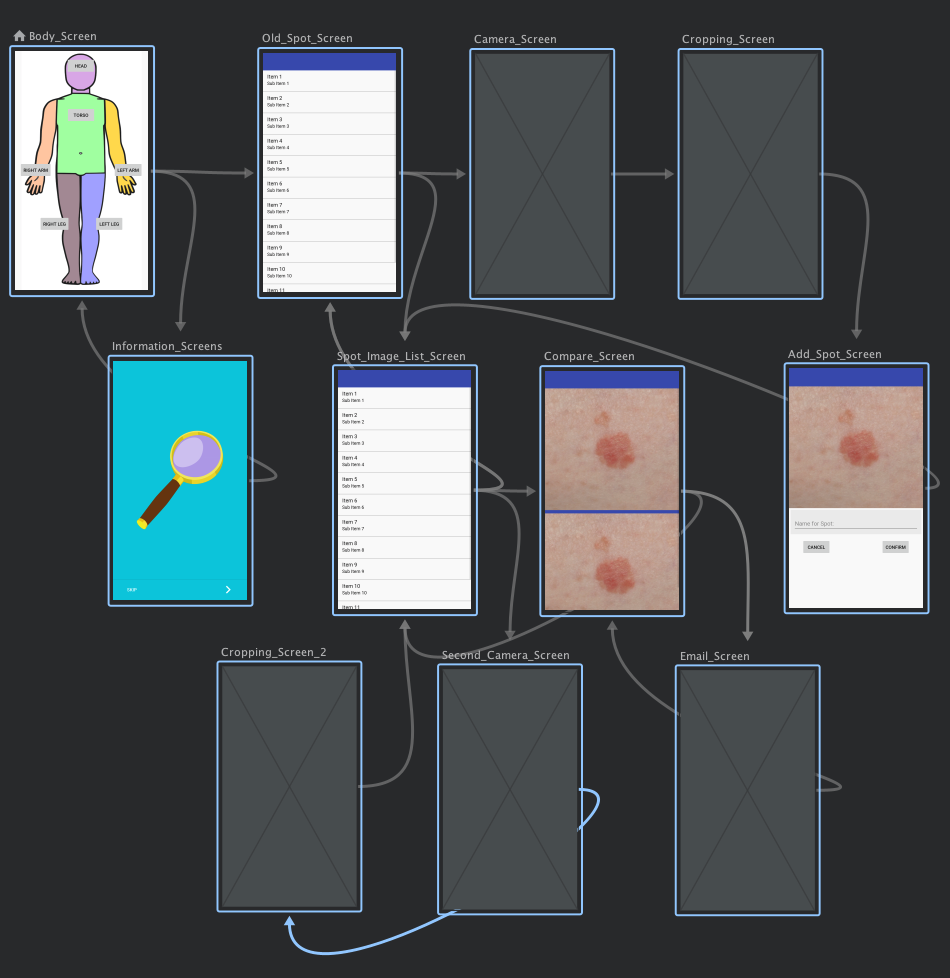
\includegraphics[width=1.2\textwidth, center]{figures/nav_graph.png}
    \caption{Navigation Graph}
    \label{fig:nav_graph}
\end{figure}